\documentclass{acm_proc_article-sp}
\usepackage{caption}
\usepackage{listings}


\begin{document}

\title{"Bar Dude" \\ An Interactive Bar}

\numberofauthors{4} 
\author{
\alignauthor
Nicolas Erbach\\
       \email{s9nierba@stud.uni-saarland.de}
\alignauthor
Tobias Kiefer\\
       \email{s9tskief@stud.uni-saarland.de}
\and
\alignauthor Maike Maas\\
       \email{s9memaas@stud.uni-saarland.de}
\alignauthor Manuel Zapp\\
       \email{s9mazapp@stud.uni-saarland.de}
}
\date{25 September 2015}

\maketitle

\section{Introduction}
With the upcoming LED technology and its numerous advantages, new possibilities especially for the maker scene emerged. Due to their low costs LEDs are affordable for nearly all DIY projects. Their low energy consumption and low operation voltage make them easily accessible also for non electronic experts with micro controller boards like the Arduino.\\
In the seminar "Affective Lighting" the participants are encouraged to build their own project by combining interactive LED lighting and affective computing to create environmental responsive lighting experiences for future smart environments. The goal is the design and development of a system or devices that can recognize, interpret, and process human affects to adapt the lighting environment accordingly. The whole seminar is organized as an hackathon in teams of usually four person. This document guides the reader throughout the creation process of ``Bar Dude" an interactive bar. ``Bar Dude" is a system that uses different light signals to lead a user through the mixing procedure of the selected cocktail.

\section{Concept}
In this section we describe the thought process from the rough idea of a interactive bar using LED technology over our design phase till a concrete plan of ``Bar Dude" an interactive bar.
\subsection{Idea}
With the enormous amount of different cocktails it is unfeasible for non-bartenders to know how to mix every cocktail properly. ``Bar Dude" addresses this problem by guiding people through the single steps of mixing their favorite cocktails. In a first step users are able to choose a cocktail from a proper interface. In a second step the user is advised to perform different action of the mixing procedure by illuminating the ingredients of the cocktail or displaying various light animations.
\subsection{Design}

In a first step we planed the shape of the bar using Adobe Inventor as shown in figure \ref{fig:bar_inventor}. One of our goals was to provide as many cocktails as possible with least ingredients. Regarding our calculations twelve ingredients is the best trade-off and gave us circa 50 different cocktails. This is why we designed it with two plexiglass shelves each with room for six bottles. Under the lowermost shelf we planed to place the cocktail glasses, the ice bucket and the cocktail shaker. LED strips should be used to illuminate the ingredients and should be arranged properly behind the plexiglass shelves. 

\begin{minipage}{\linewidth}% to keep image and caption on one page
\makebox[\linewidth]{%        to center the image
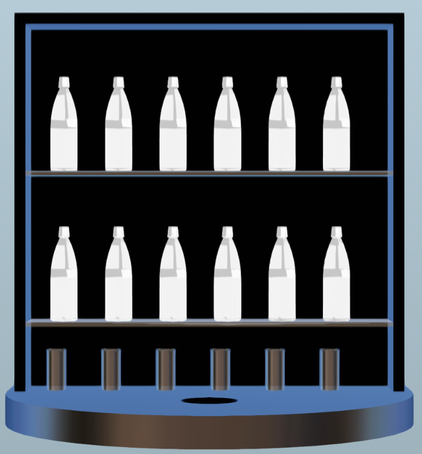
\includegraphics[width=0.5\linewidth]{pictures/bar_inventor.png}}
\captionof{figure}{Sketch of the bar}\label{fig:bar_inventor}%      only if needed  
\end{minipage}

This should allow the independent illumination of each bottle. In the bottom plate of the bar, which consists of two plates with a cavity between them, a weight measuring module should be integrated so that the system is able to measure the actual amount of liquid that is already filled in the glass. To give the user visual feedback about how much liquid has to be filled in, LED strips are also placed under the weight measuring module. Furthermore the cavity of the bottom plate makes it possible to stow all electronics inside the bar so that the user does not see any wiring unless the raspberry pi surface. On this surface we want to give little instructions for each step in the mixing process of the selected cocktail.

Our shopping list looks as follows:
\begin{itemize}
\item Raspberry Pi 2 B
\item Raspberry LCD display
\item Power supply for Raspberry Pi
\item SD-card for Raspberry Pi
\item WLAN adapter for Raspberry Pi
\item weight measuring module
\item Arduino Uno
\item Power supply for Arduino Uno
\item Adafruit Neopixel 120 LED
\item Plexiglass
\item Wood
\item USB cable for connection between Raspberry Pi and Arduino
\end{itemize}
\begin{figure}[htbp] 
  \centering
     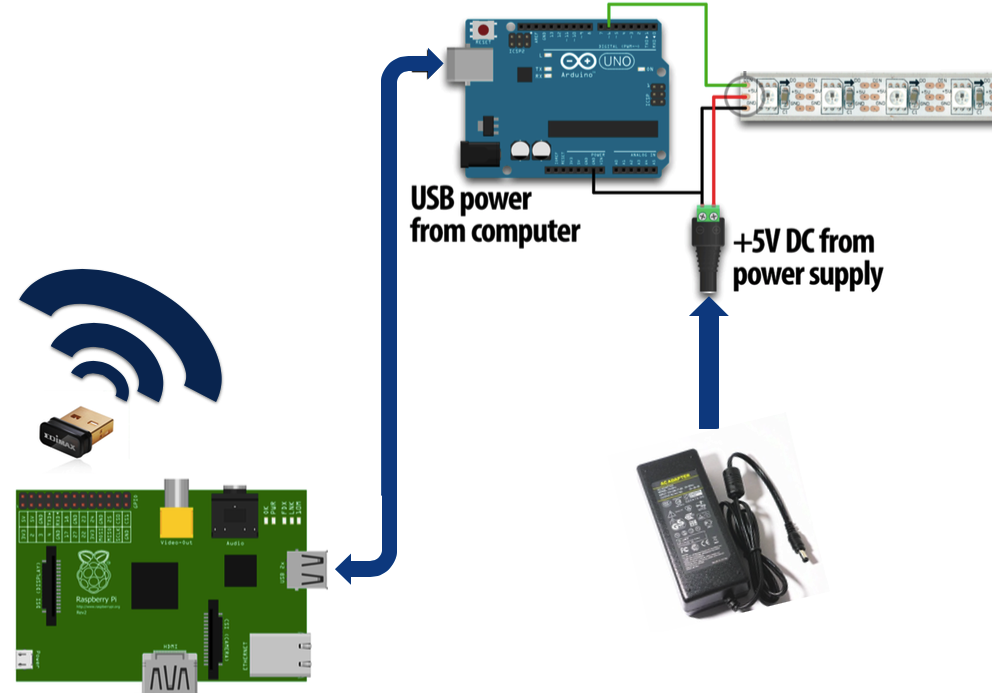
\includegraphics[width=0.7\linewidth]{pictures/technical.png}
  \caption{Technical sketch}
  \label{fig:technical}
\end{figure}

In the first technical sketch (figure \ref{fig:technical}) we used a Raspberry Pi spanning a WiFi network and running a web server providing the user interface of the bar. This Raspberry Pi is connected via a serial connection over a USB cable to a Arduino Uno. To this micro controller the LED strips and the weight measuring module are connected.

\section{Hardware Construction}
In this section we explain the hardware construction process. In the first part a detailed description of the woodwork is given. After that the design and realization of the plexiglass shelves is stated.

\subsection{Woodwork}
After planning the rack and the shelves of the bar, we calculated the amount of wood we would need to build it. In a next step we had to cut the wood we bought into the right pieces.

\begin{minipage}{\linewidth}% to keep image and caption on one page
\makebox[\linewidth]{%        to center the image
  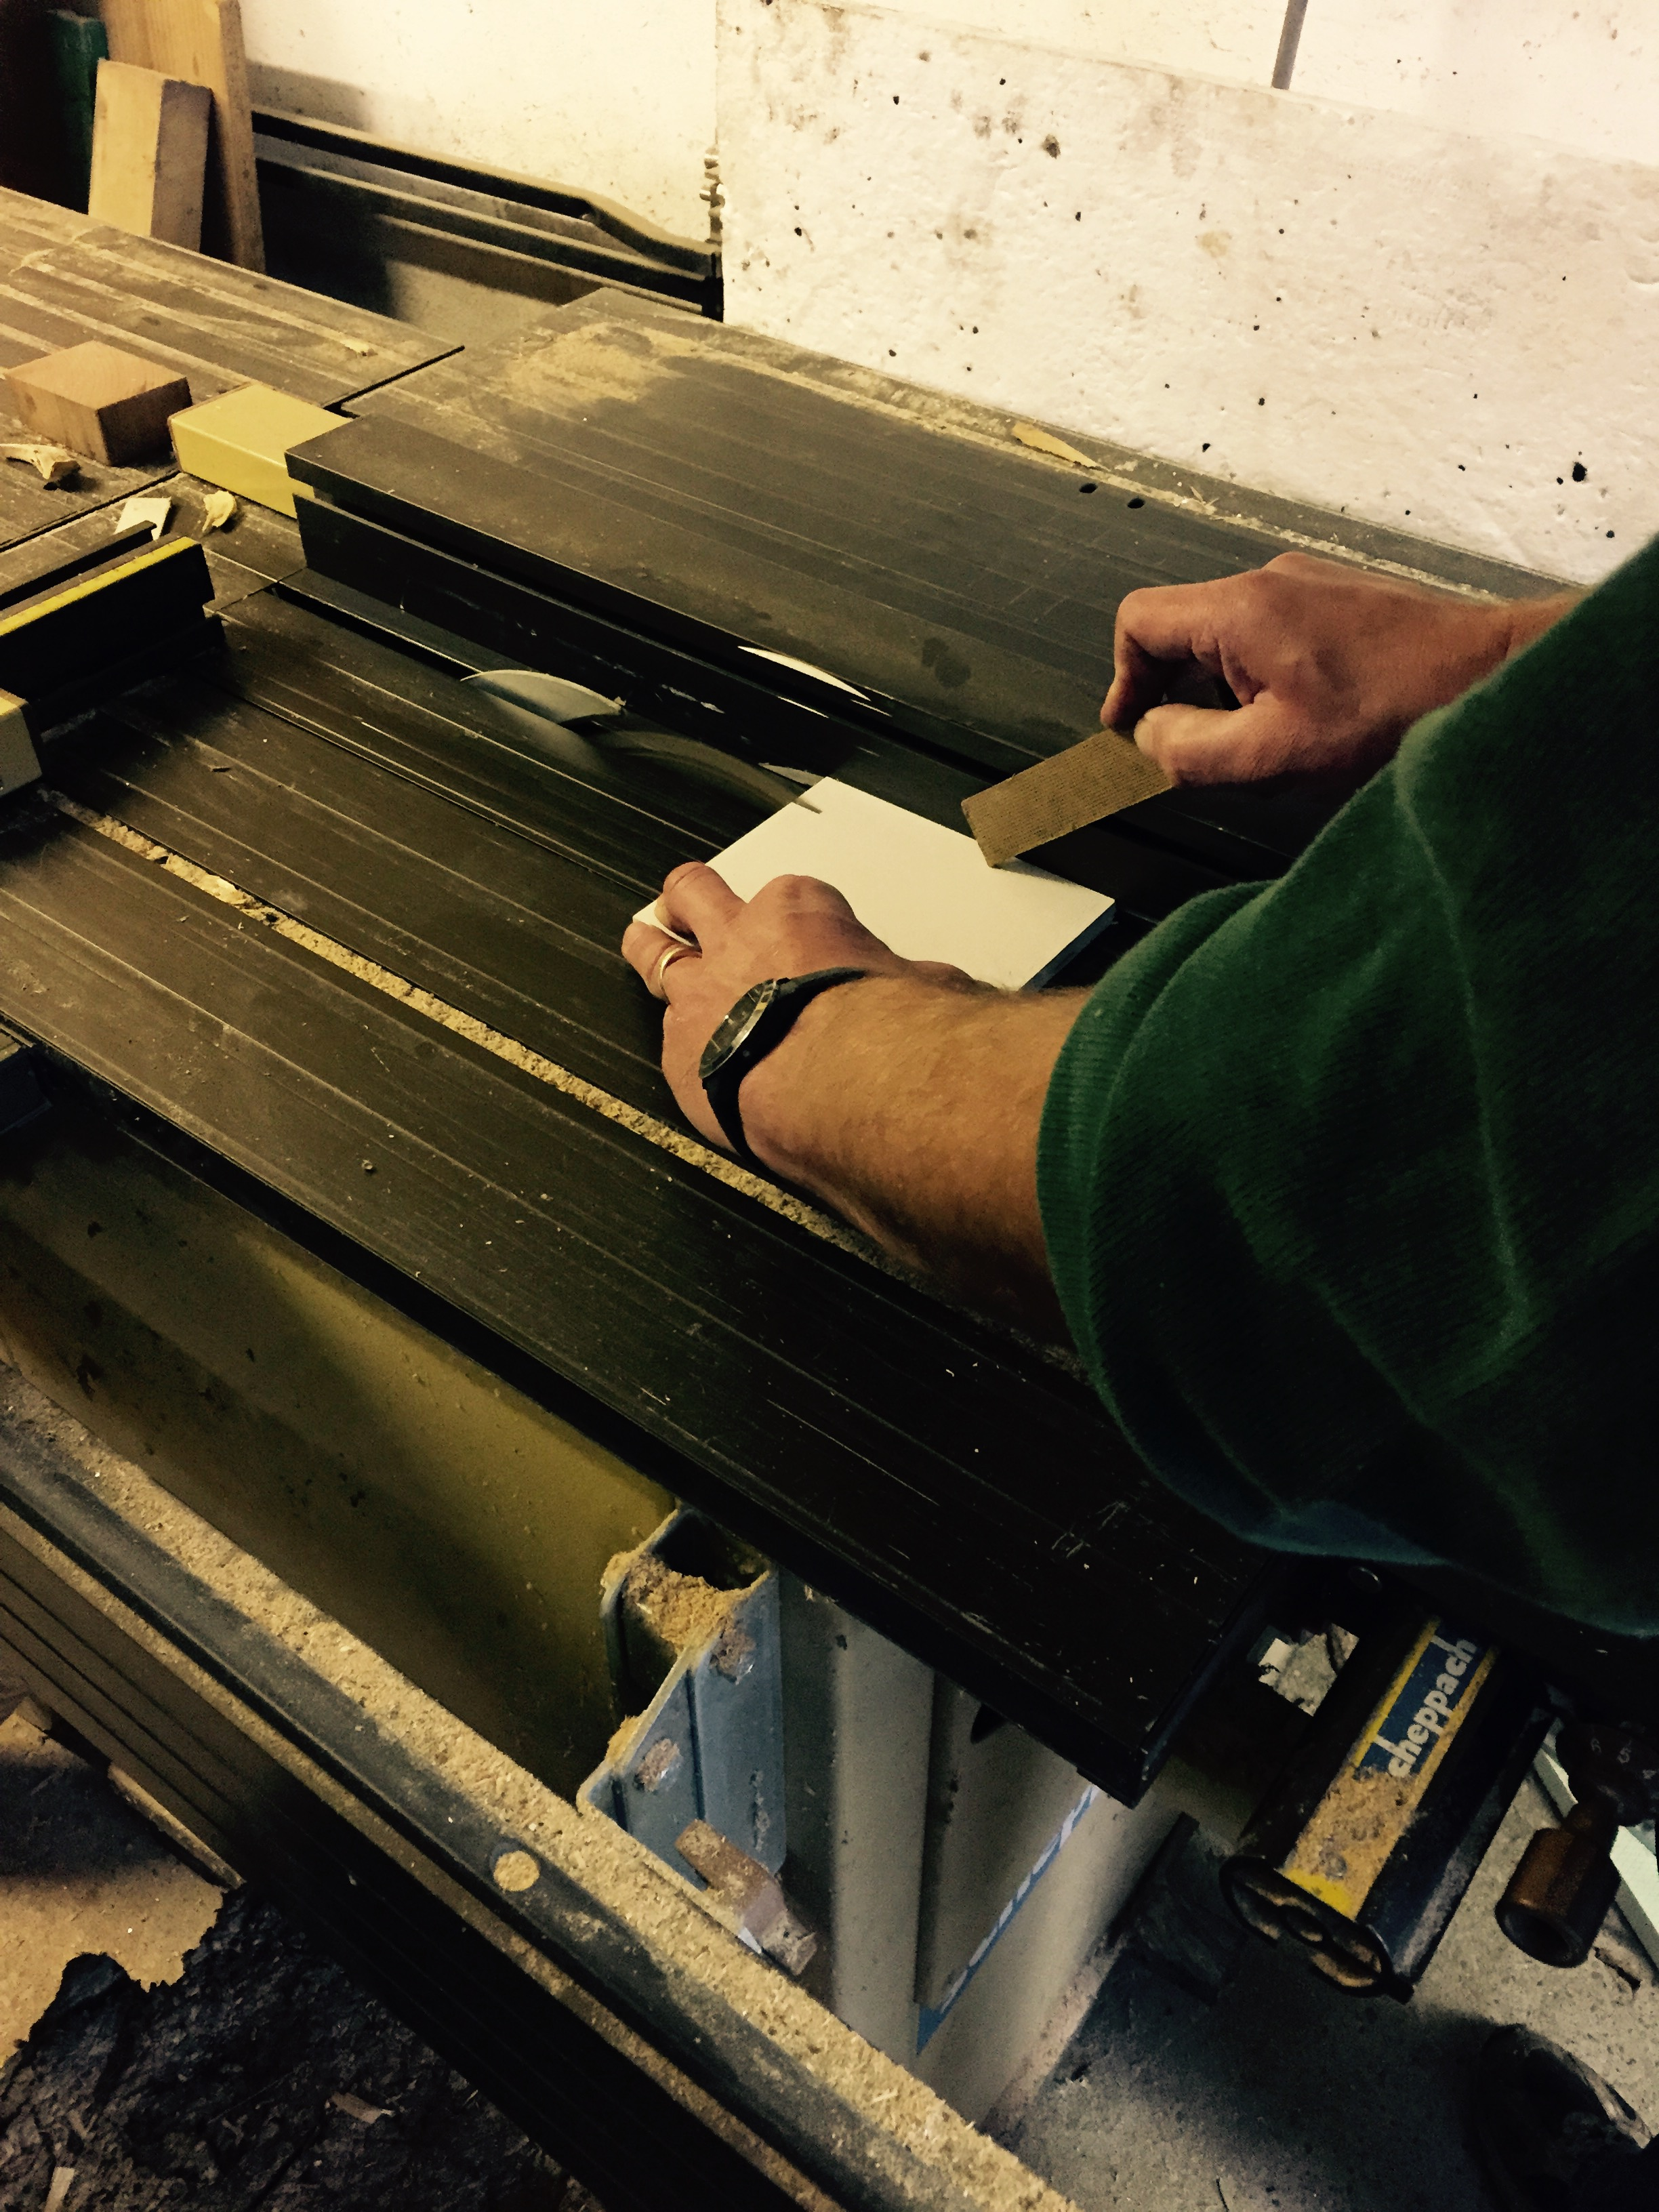
\includegraphics[width=0.7\linewidth]{pictures/cutting_wood.jpg}}
\captionof{figure}{Cutting of the wood}\label{fig:cutting_wood}%      only if needed  
\end{minipage}


For the rounding of the rack bottom we contacted a local carpenter who did the difficult rounding cuts using a cnc mill. The other small pieces were cut with a buzz saw as you can see in figure \ref{fig:cutting_wood}.

\begin{minipage}{\linewidth}% to keep image and caption on one page
\makebox[\linewidth]{%        to center the image
  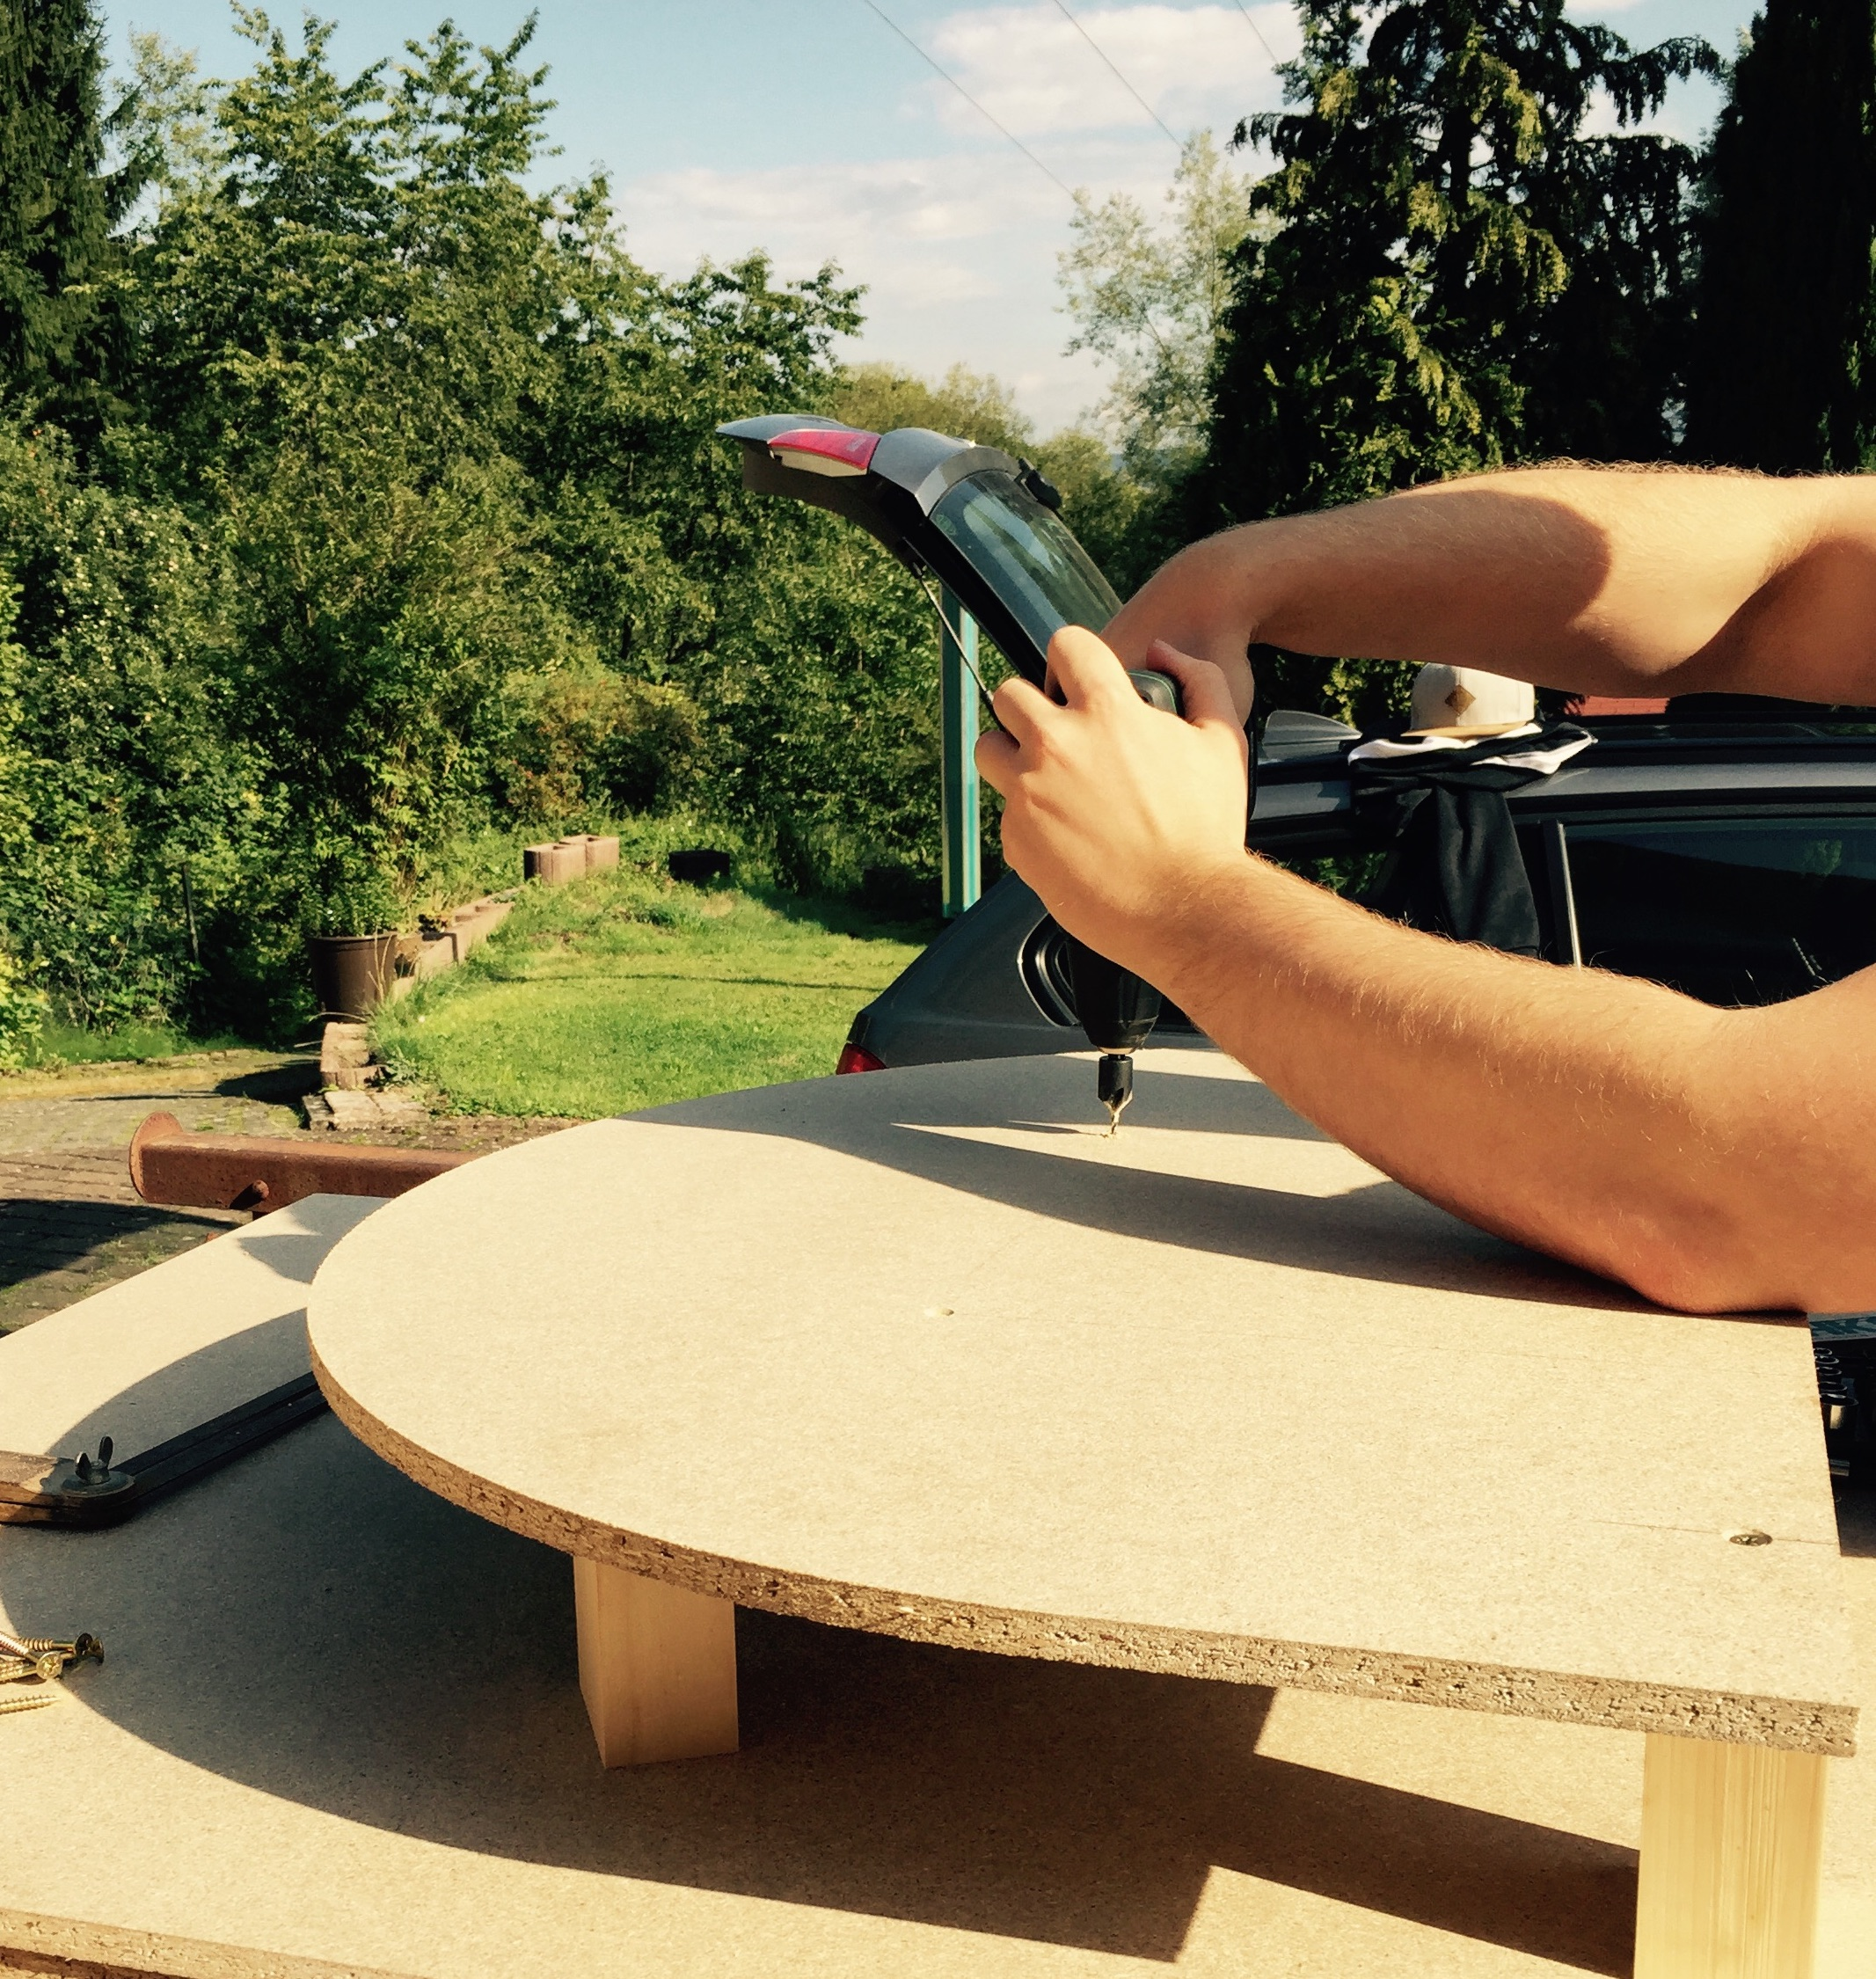
\includegraphics[width=0.6\linewidth]{pictures/assembling.jpg}}
\captionof{figure}{Assembling of the rack}\label{fig:assembling}%      only if needed  
\end{minipage}

When all pieces of the rack were fitted, we started to assemble the rack. For assembly we used screws and wood glue so that the bar would keep stable. Figure \ref{fig:assembling} shows how the base plate is screwed together.

\begin{minipage}{\linewidth}% to keep image and caption on one page
\makebox[\linewidth]{%        to center the image
  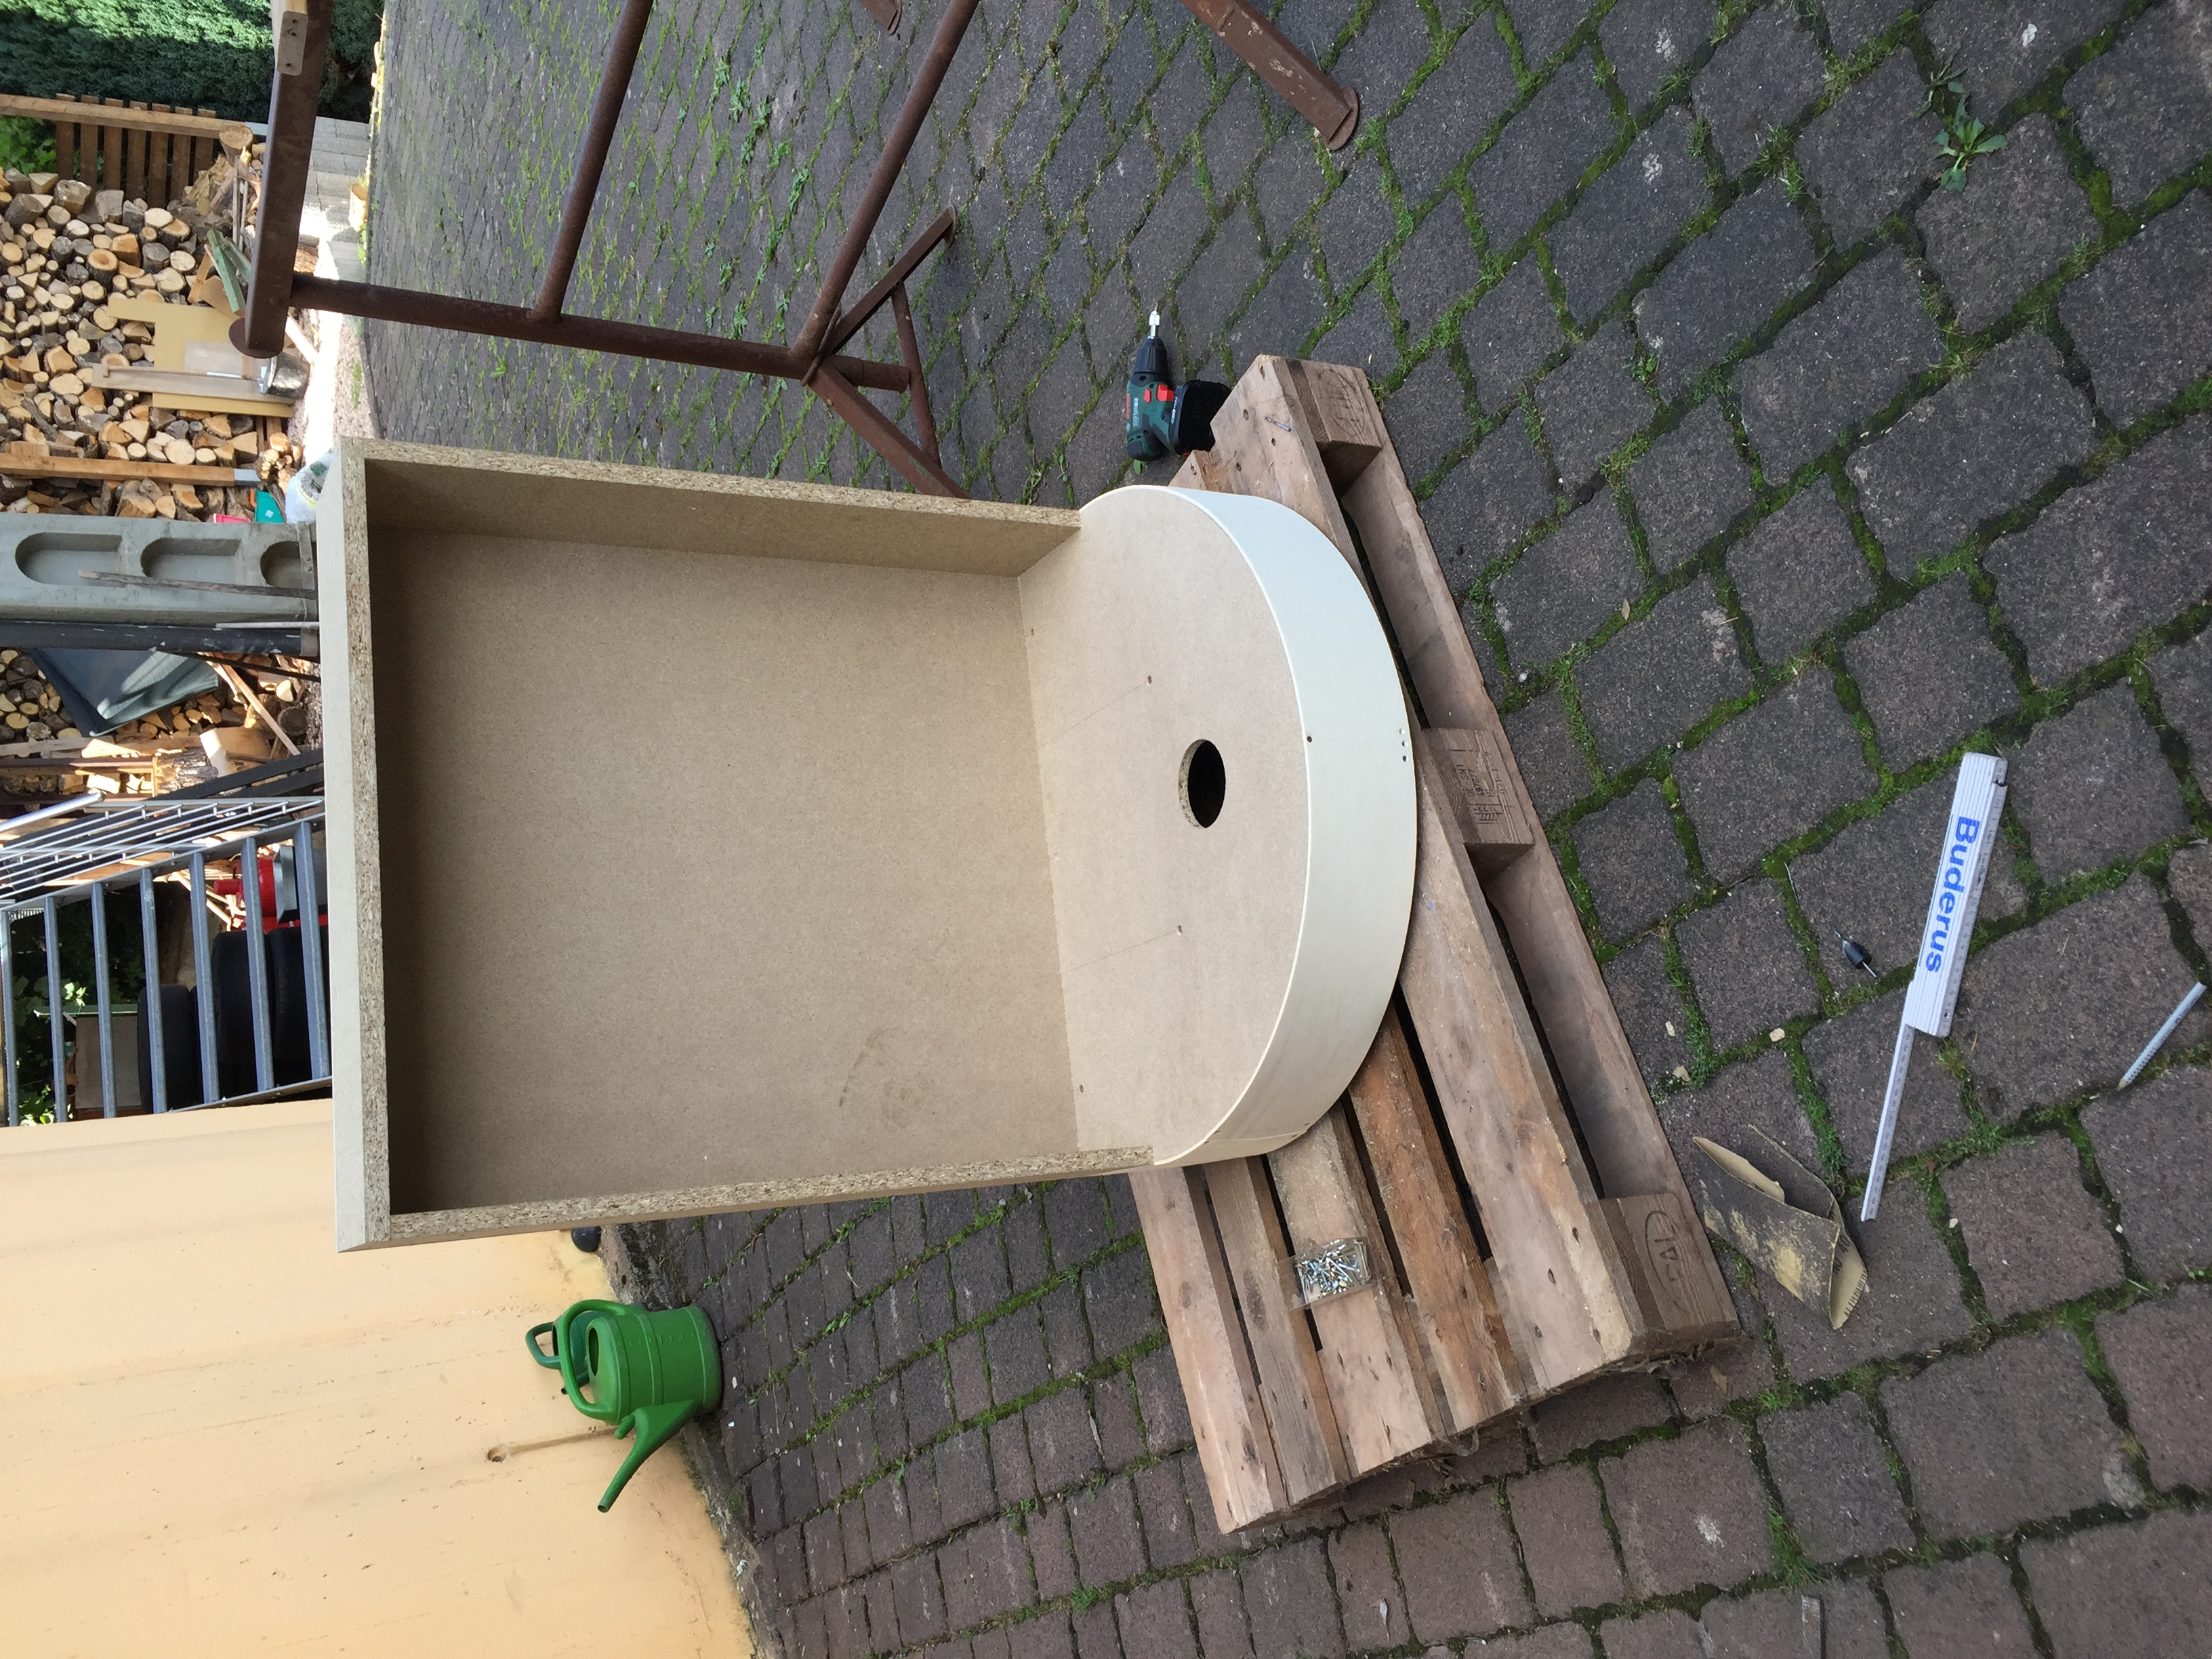
\includegraphics[width=0.6\linewidth, angle =270]{pictures/rack2.jpg}}
\captionof{figure}{Framing of the rack}\label{fig:framing}%      only if needed  
\end{minipage}


The finished framing of the rack is shown in figure \ref{fig:framing}. This picture also illustrates that we did the panelling between the two base plates with 4 mm poplar wood because this is thin and flexible so that it can be bend.

\begin{minipage}{\linewidth}% to keep image and caption on one page
\makebox[\linewidth]{%        to center the image
  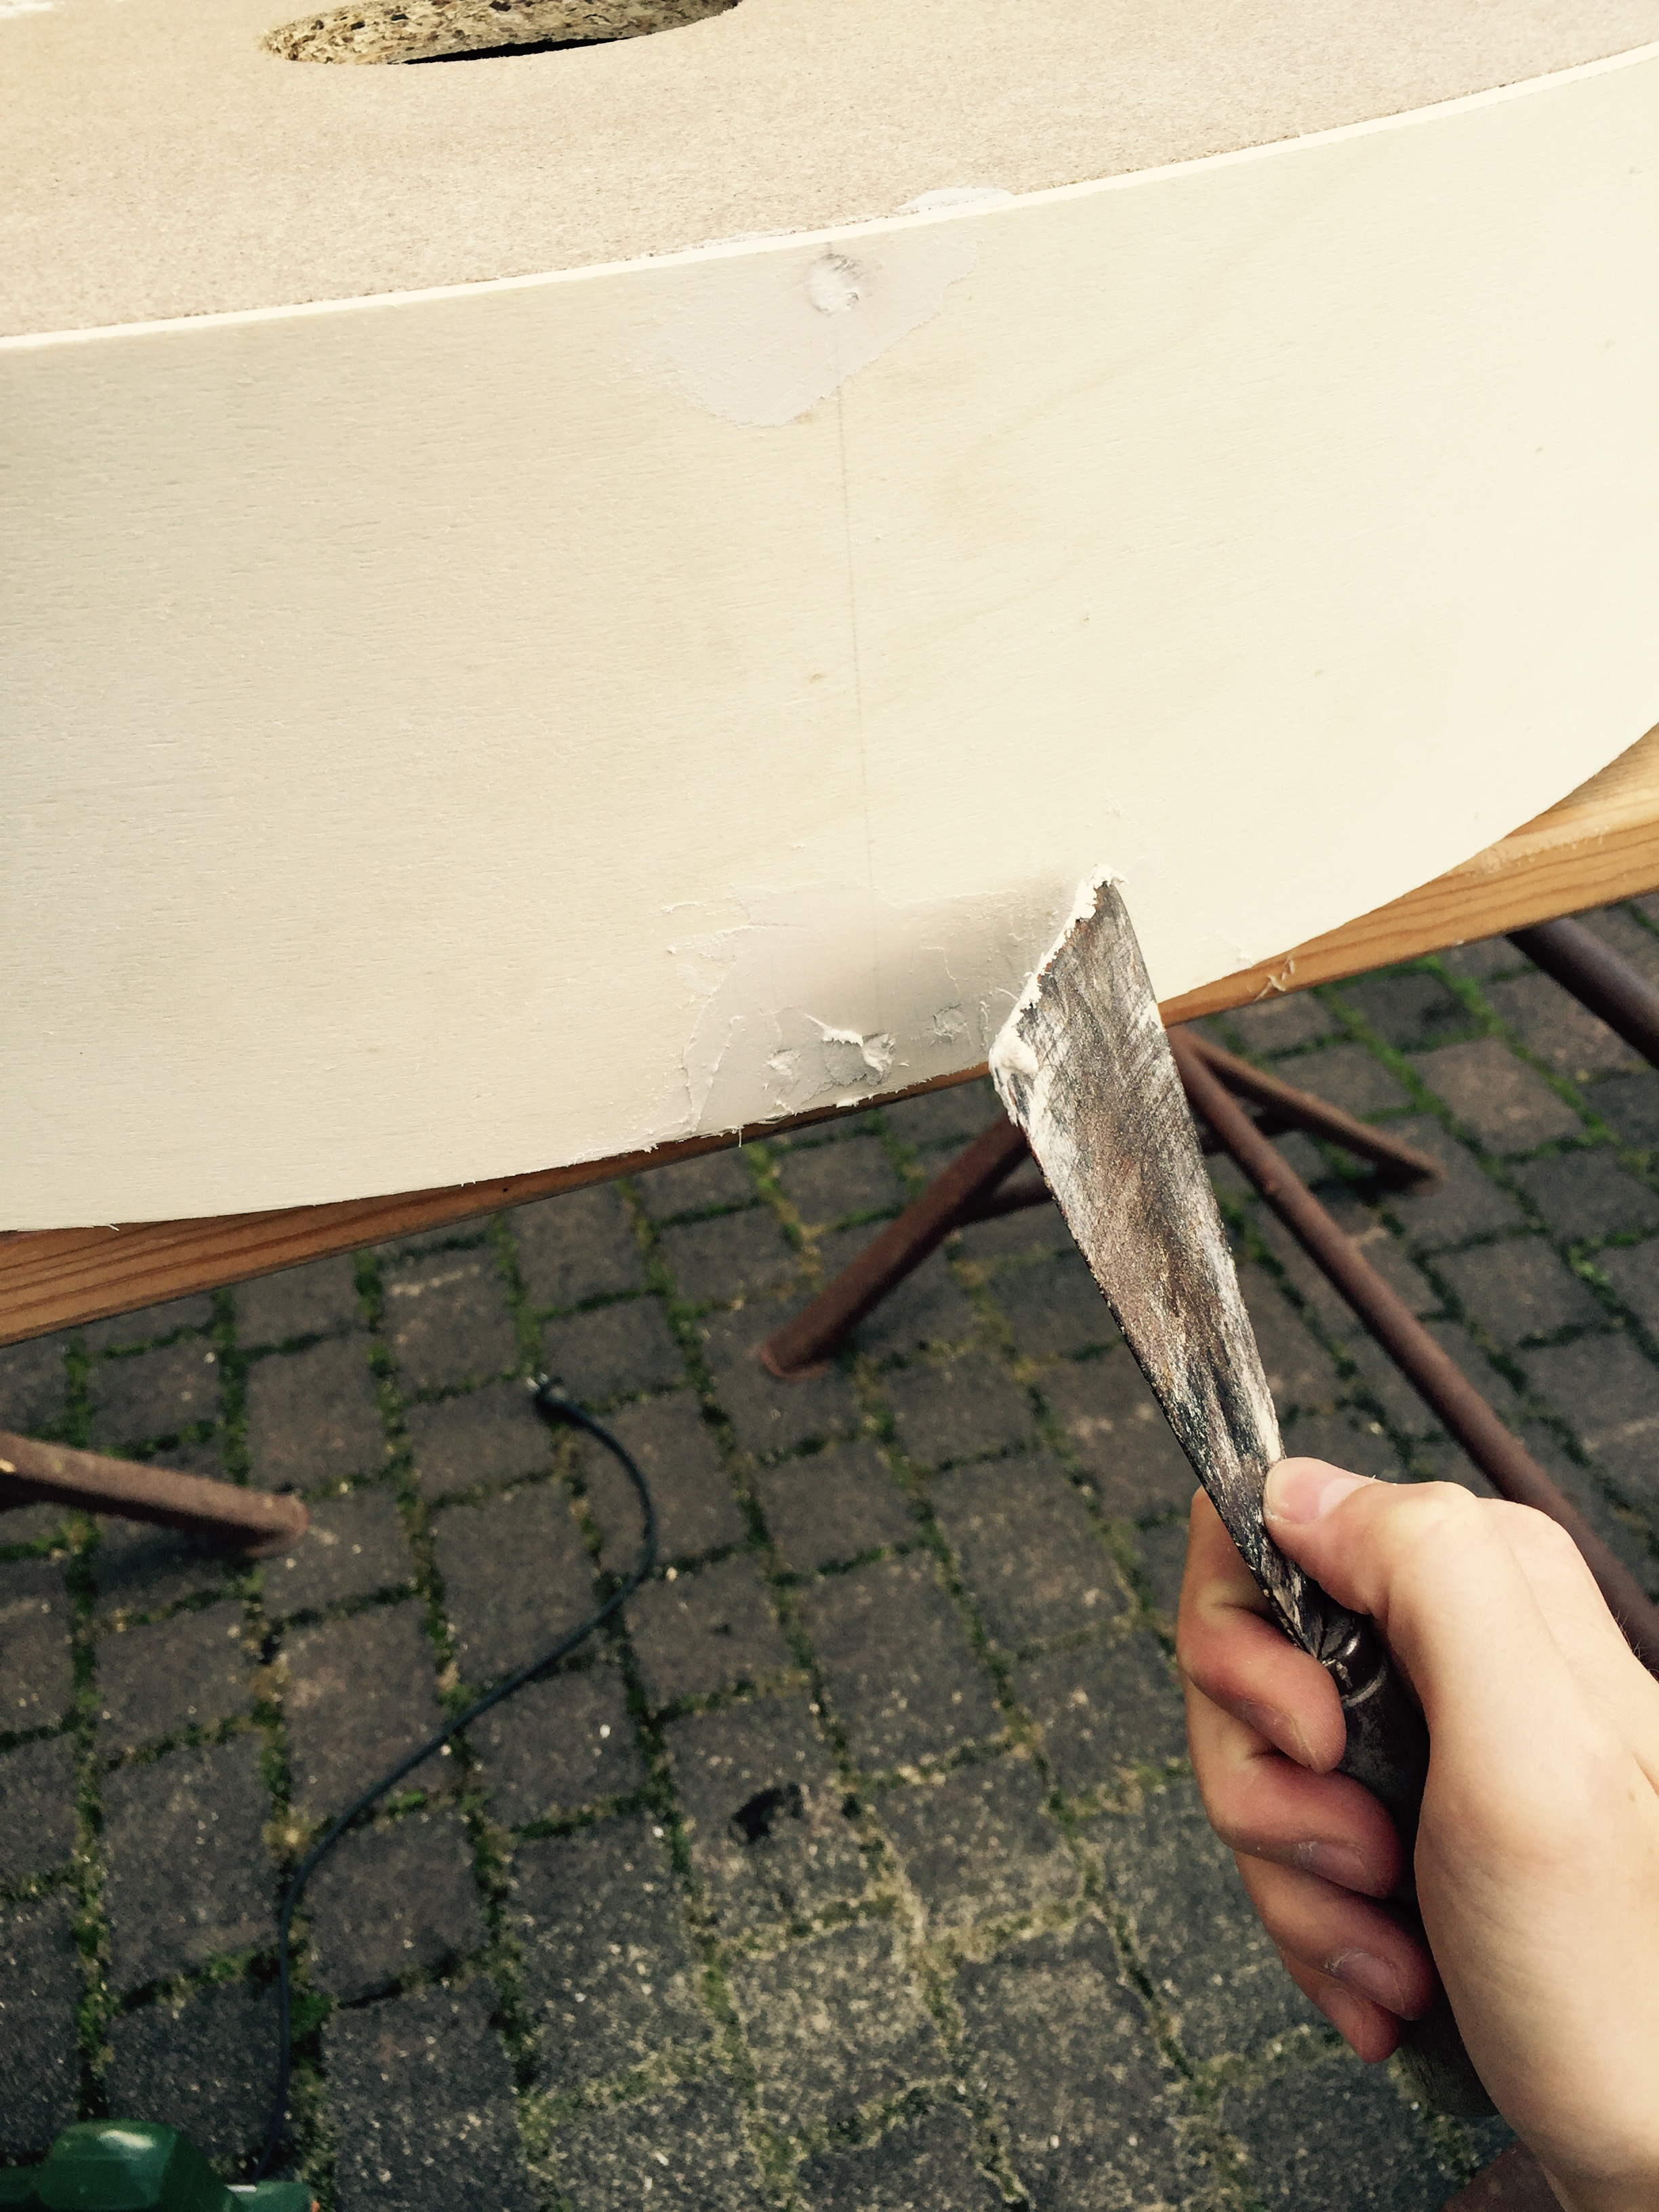
\includegraphics[width=0.55\linewidth]{pictures/filling.jpg}}
\captionof{figure}{Filling of the screw wholes}\label{fig:filling}%      only if needed  
\end{minipage}


For deriving a smooth surface of the rack, we filled all screw wholes with filling paste. Since we used chipboard, we also filled the edges of the rack, so that it is easier to prime and paint the bar. 

\begin{minipage}{\linewidth}% to keep image and caption on one page
\makebox[\linewidth]{%        to center the image
  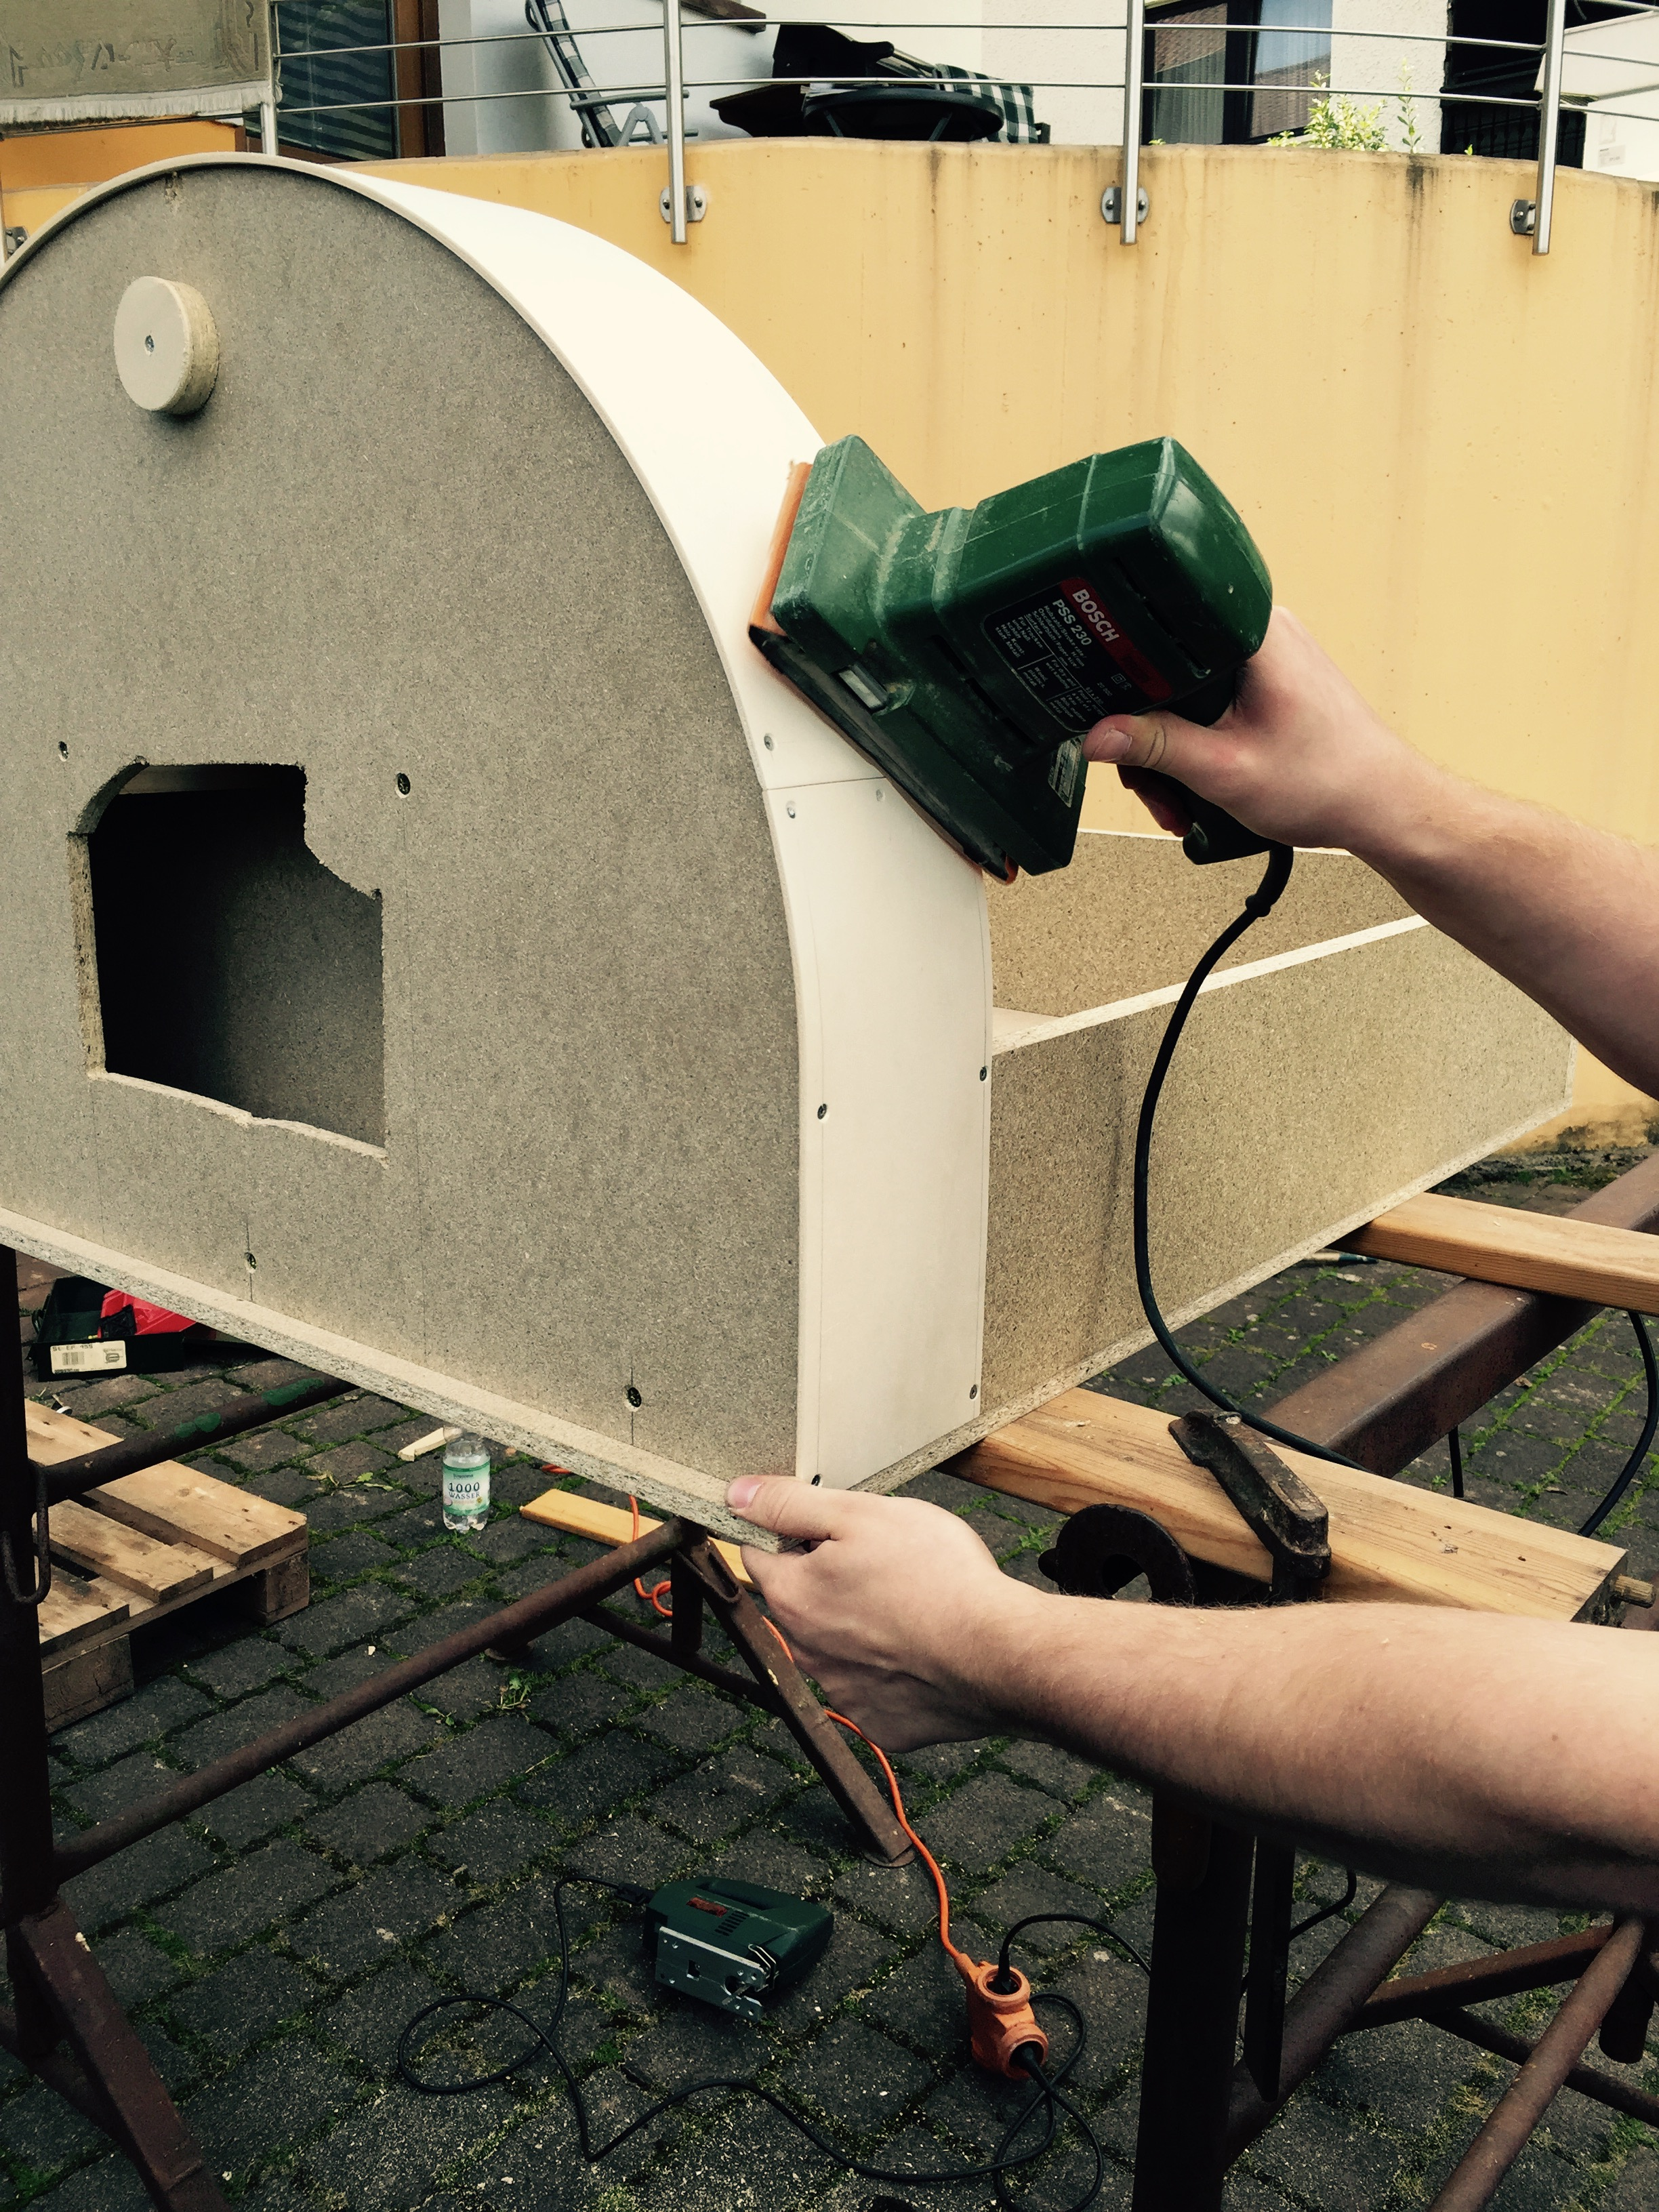
\includegraphics[width=0.45\linewidth]{pictures/polishing.jpg}}
\captionof{figure}{Polishing the rack}\label{fig:polishing}%      only if needed  
\end{minipage}


In a next step we polished the bar since we had to remove the superfluous filling paste and roughened the wood. This work step can be seen in figure \ref{fig:polishing}

\begin{minipage}{\linewidth}% to keep image and caption on one page
\makebox[\linewidth]{%        to center the image
   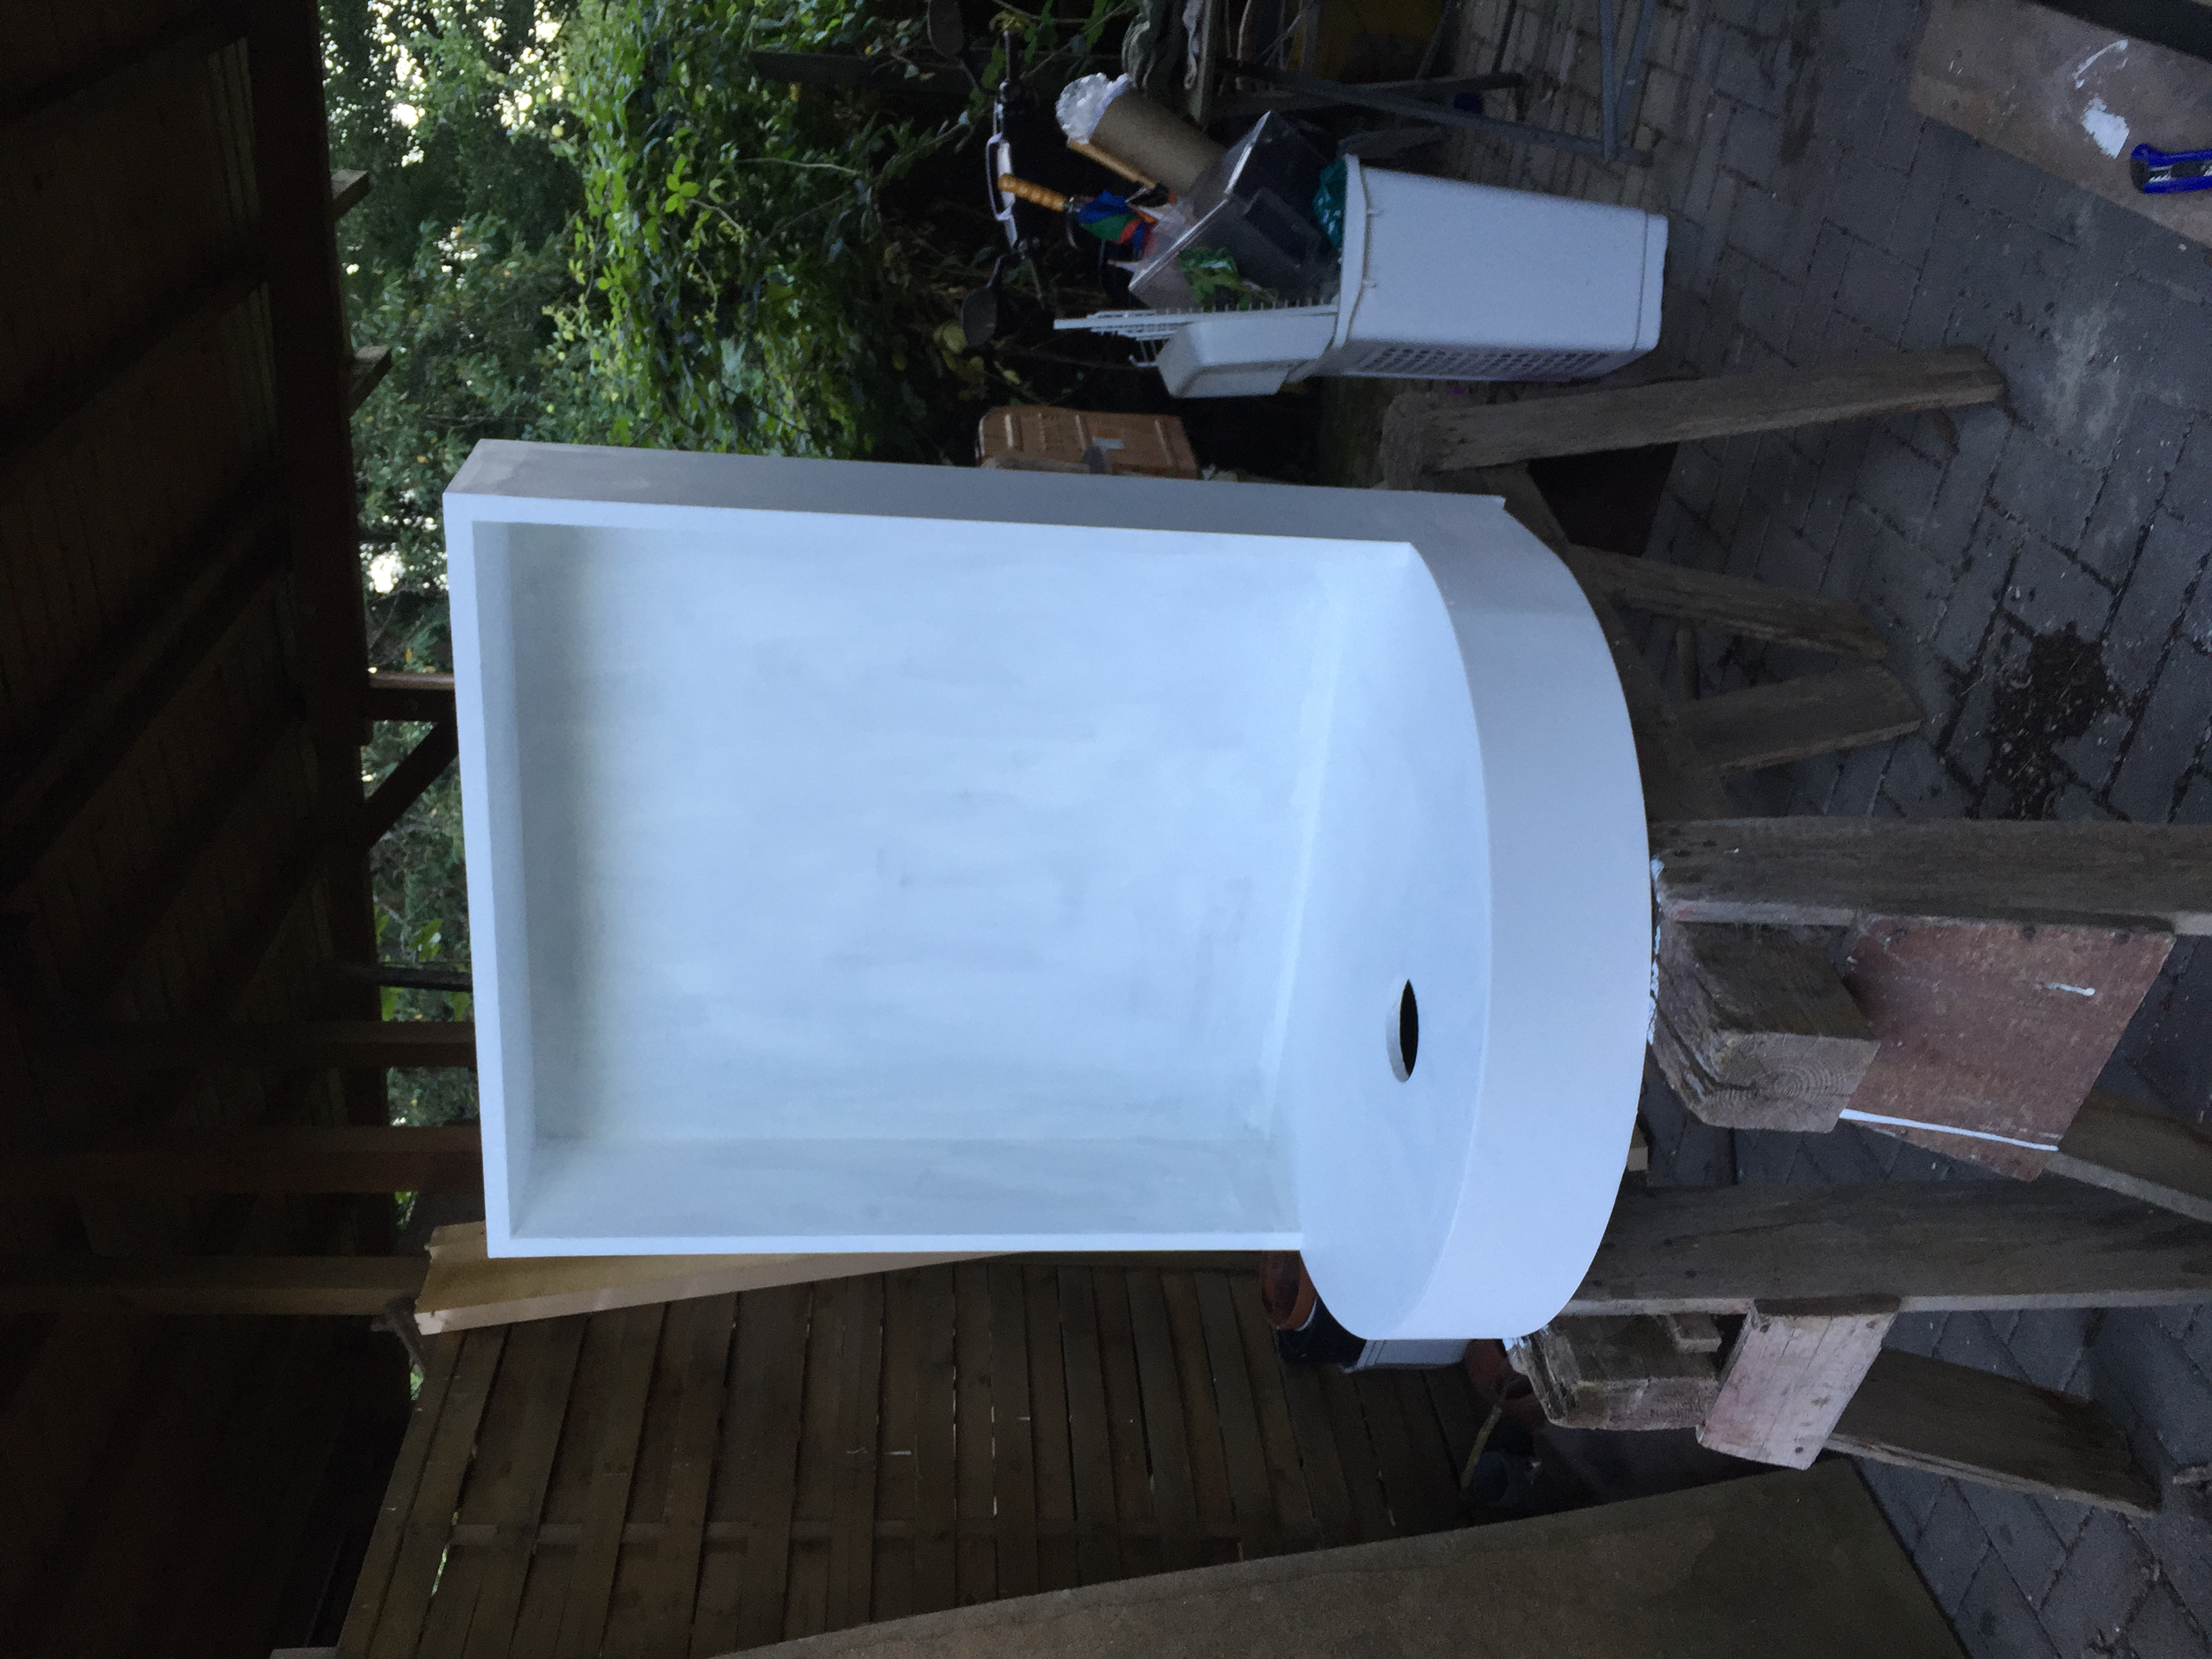
\includegraphics[width=0.6\linewidth, angle =270]{pictures/rack3.jpg}}
\captionof{figure}{The primed rack}\label{fig:priming}%      only if needed  
\end{minipage}
 

After polishing and cleaning the rack with compressed air, we were able to prime the rack. This is important since primer creates a smooth and consistent layer for the painting.


\subsection{Plexiglass Shelves}
The initial design planed that the two shelves only consisted of two full plexiglass plates.

\begin{minipage}{\linewidth}% to keep image and caption on one page
\makebox[\linewidth]{%        to center the image
   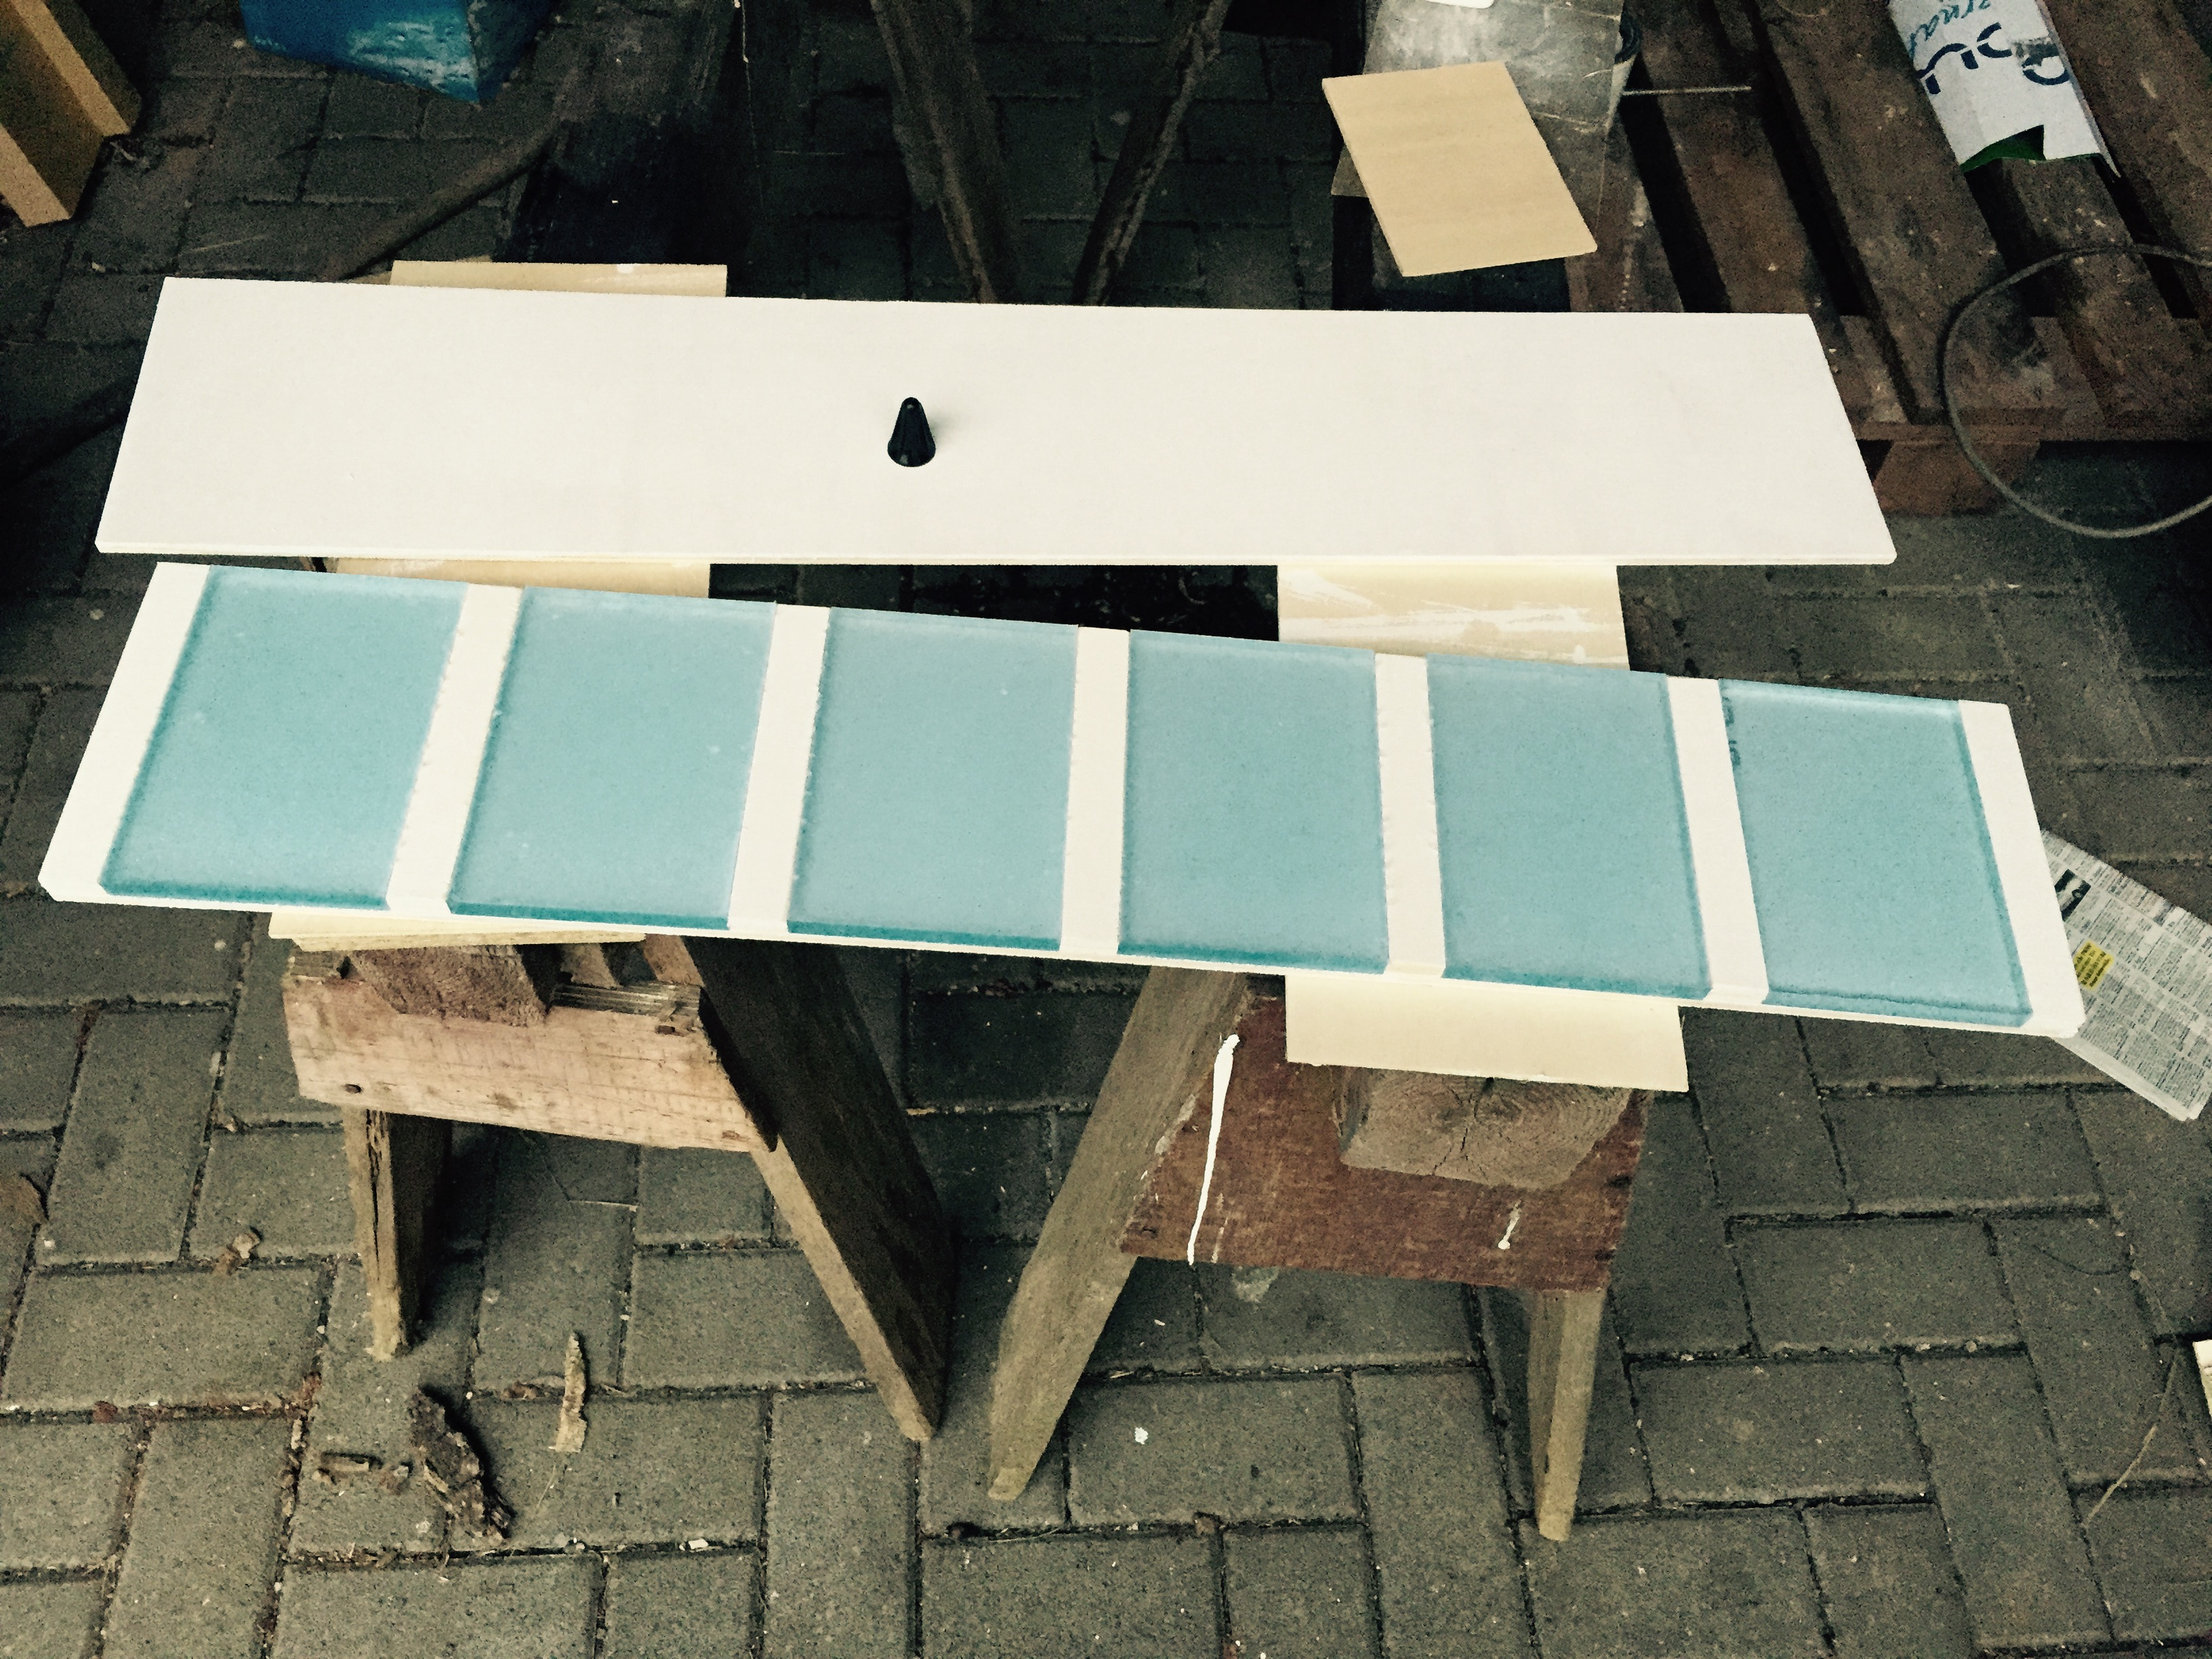
\includegraphics[width=0.5\linewidth]{pictures/plexiglass.jpg}}
\captionof{figure}{Building the shelves}\label{fig:building_shelves}%      only if needed  
\end{minipage}

At the beginning of the design process we tested this approach and noticed that the illumination of the bottles was not as good as expected since the light scattered through the whole shelve when we only lighted one bottle. Therefore we redesigned the two shelves as you can see in figure \ref{fig:building_shelves}. 

\begin{minipage}{\linewidth}% to keep image and caption on one page
\makebox[\linewidth]{%        to center the image
   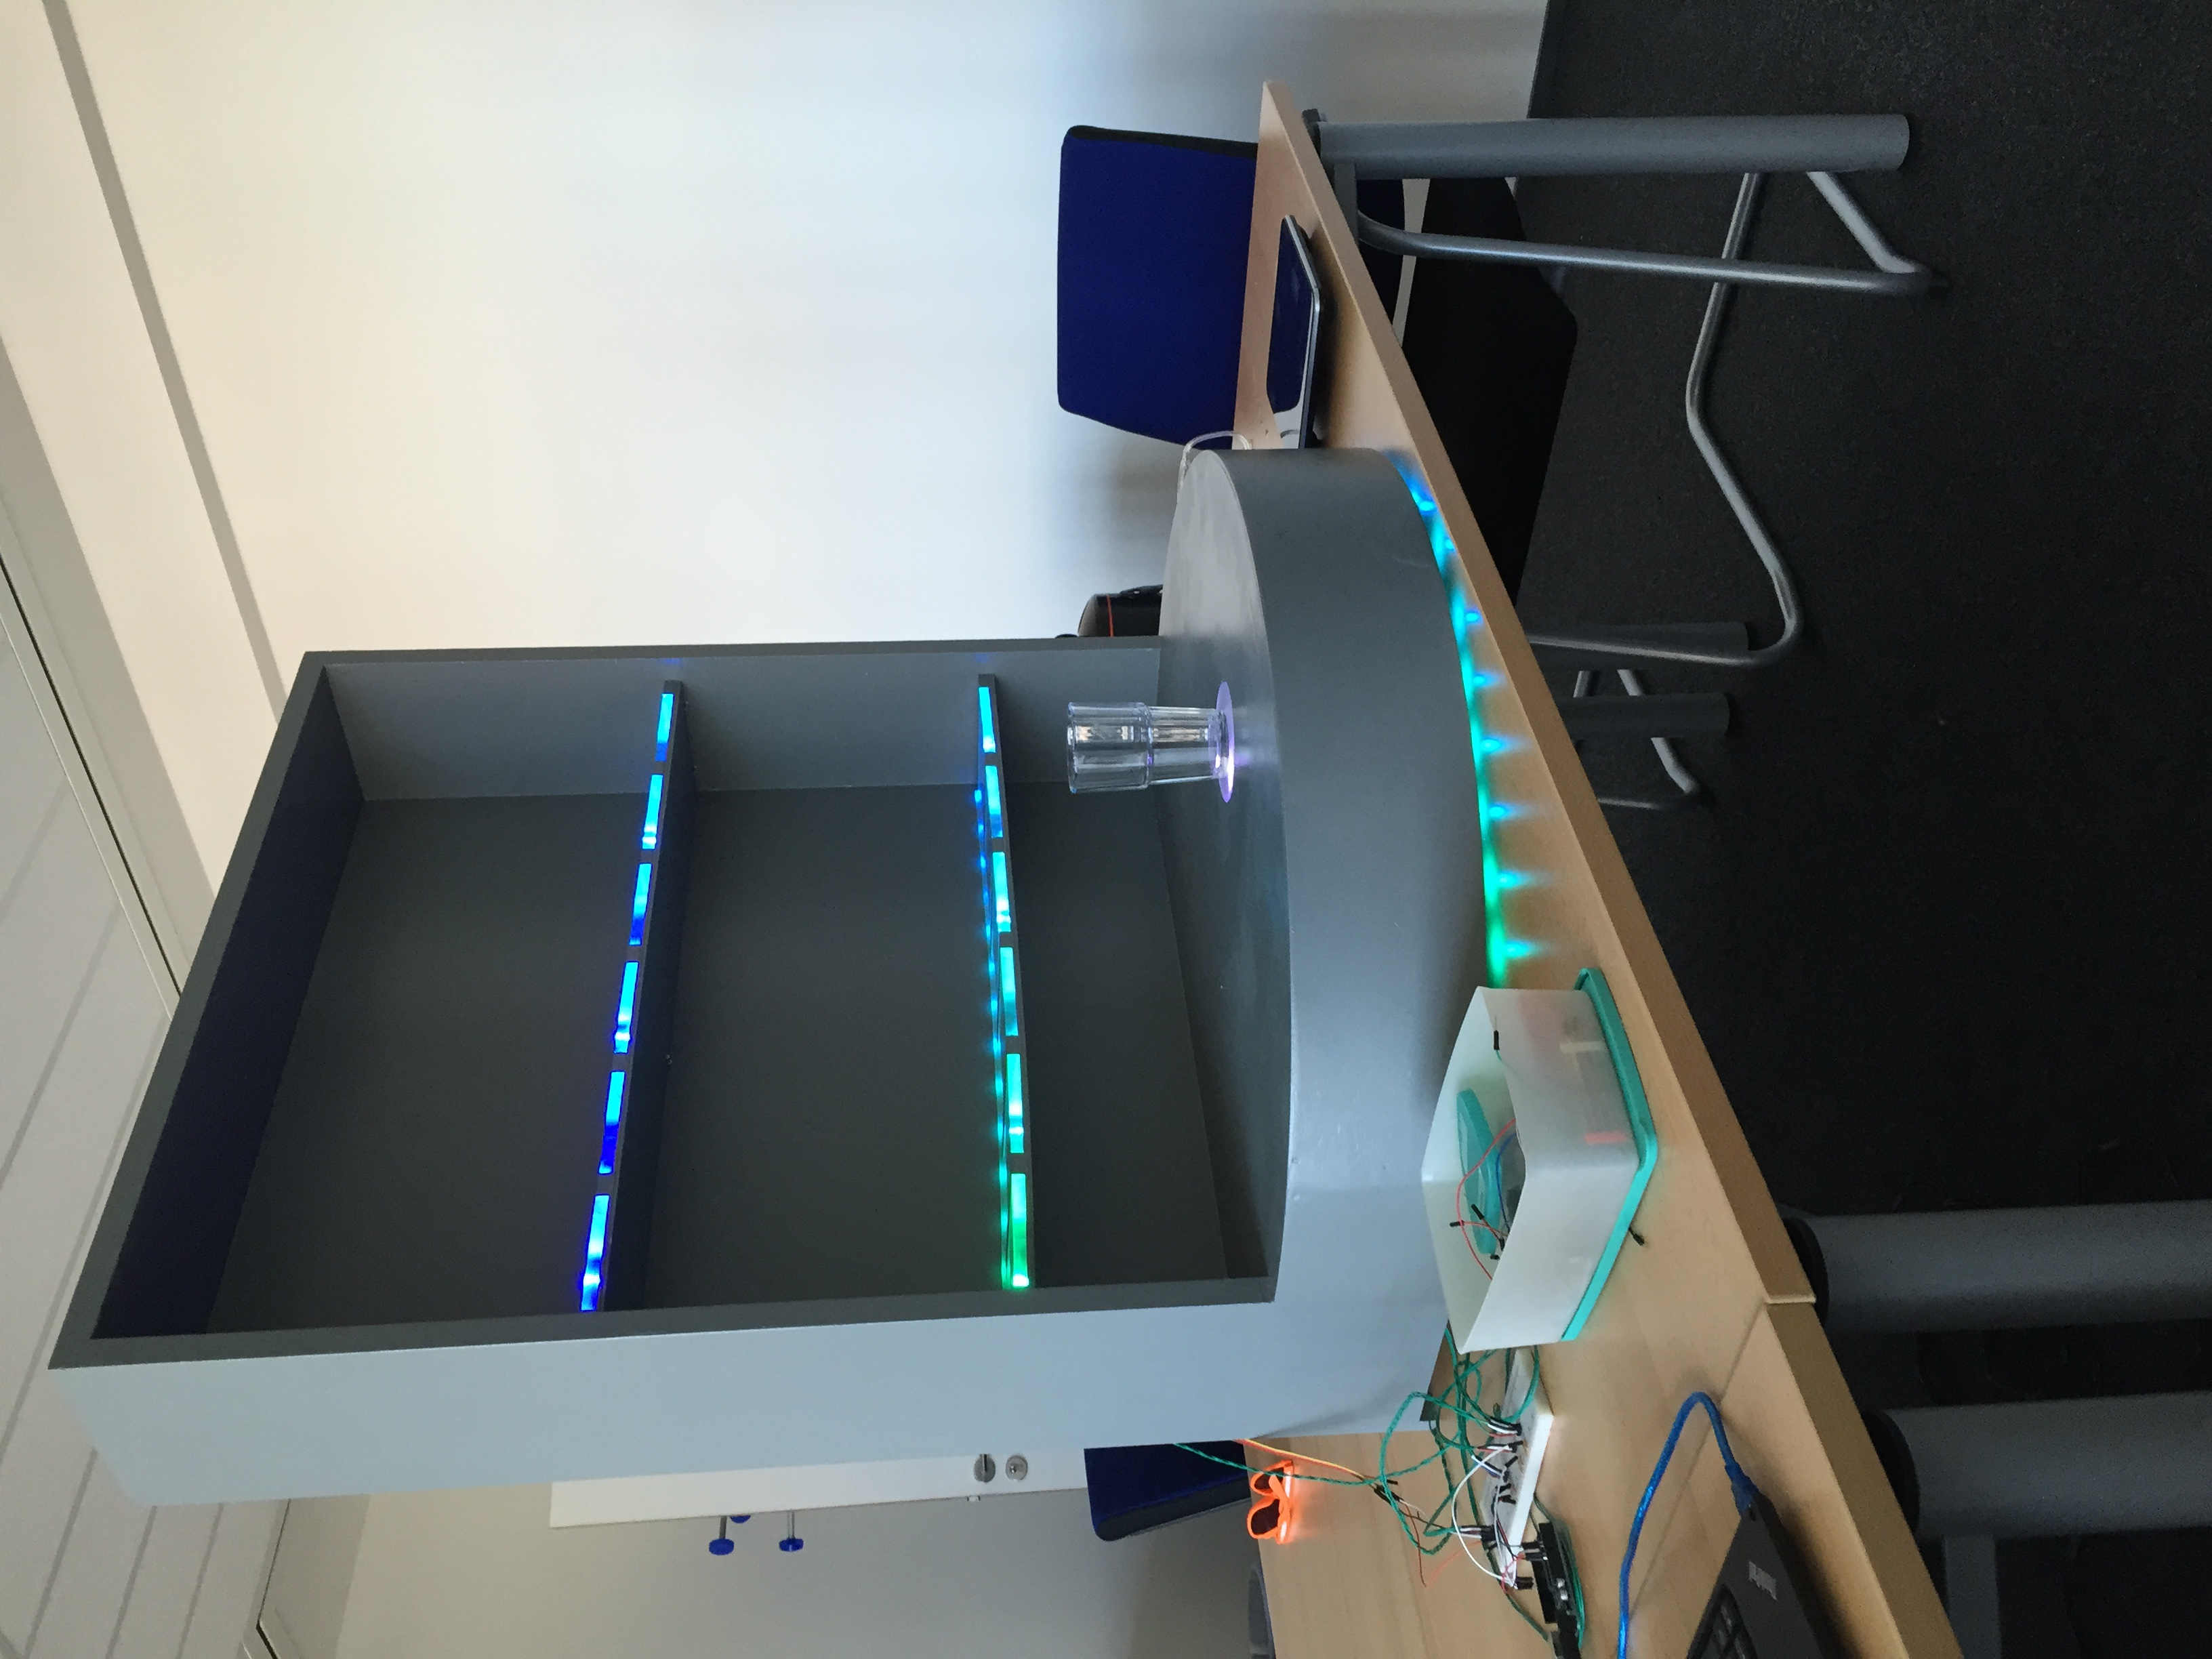
\includegraphics[width=0.7\linewidth, angle =270]{pictures/illuminated_shelves.jpg}}
\captionof{figure}{Illumination of the shelves}\label{fig:illuminated_shelves}%      only if needed  
\end{minipage}


In the new design the plexiglass plates were cut into smaller pieces and we put little pieces of wood between them. Furthermore we put a plate of wood under each shelve. This prevented the scattering of the light.\\
Figure \ref{fig:illuminated_shelves} shows the painted bar with the illumination of the shelves.

\subsection{Soldering and Wiring}
Finally we needed to connect all electronic parts together. The Raspberry Pi and the Arduino Uno are connected via an standard USB cable. Both have an individual 5 Volt power adapter with 1.2 Ampere for both devices. We have 5 LED stripes: One for both shelves, one for the glasses, one for the shaker and the ice, one for the glass panel above the scale and one for floor illumination. Each stripe needs three connections, one to ground, one to 5 Volt and one data connection to a digital pin on the Arduino board. The scale is connected to a weighting module which is also connected to ground and 5 Volt and additional to 2 analog inputs on the Arduino board.
Figure \ref{fig:fritzing} illustrates the wiring of the bar.


\begin{minipage}{\linewidth}% to keep image and caption on one page
\makebox[\linewidth]{%        to center the image
     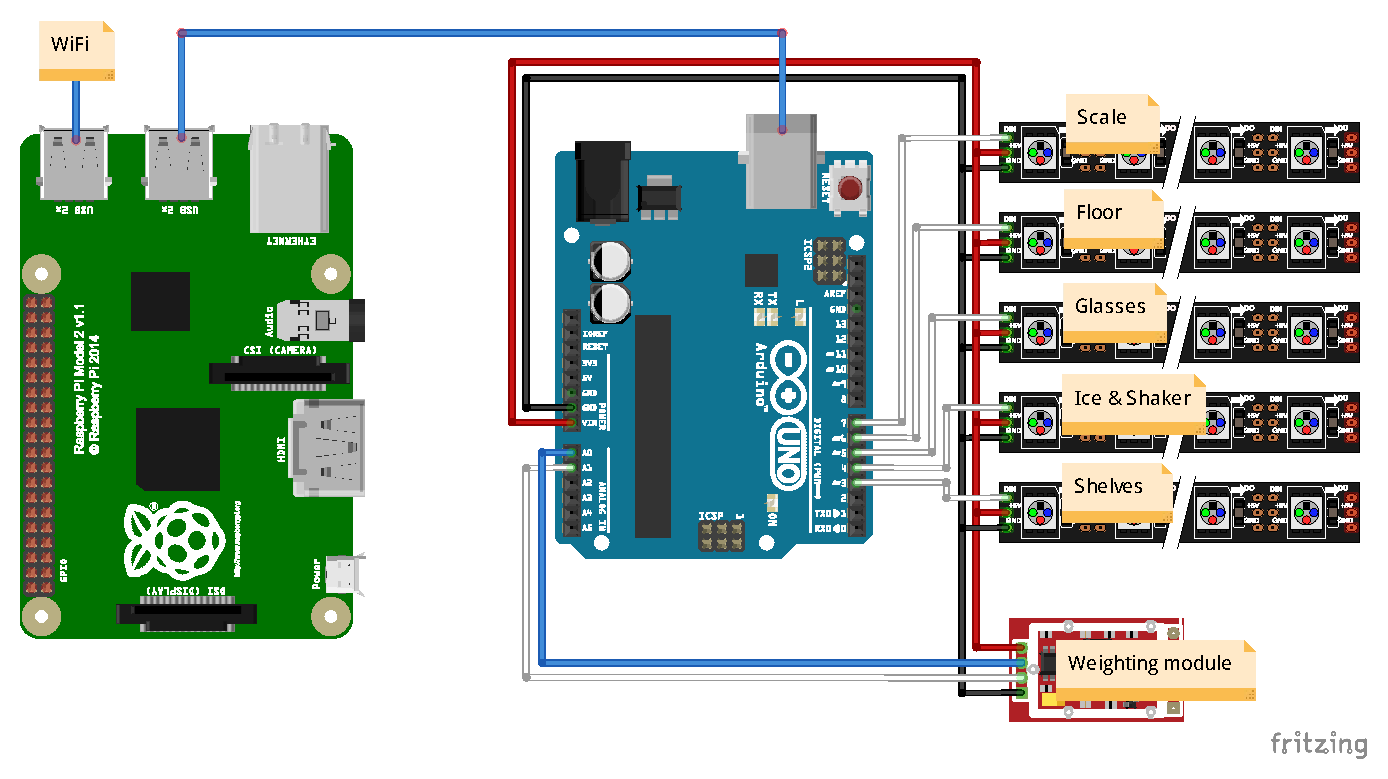
\includegraphics[width=0.8\linewidth]{pictures/sketch.pdf}}
  \captionof{figure}{Wiring sketch of the bar. The power adapters are not depicted. Made with Fritzing.}
  \label{fig:fritzing}
\end{minipage}

All cables are equipped with plugs for easier assembling. For the LED stripes they were necessary as the stripes don't fit through the drill holes. The cables from the stripes and the weighting module are all plugged into a self-soldered circuit board (see figure \ref{fig:viewfrombelow} and \ref{fig:soldering}), which is connected to the Arduino with only 3 plugs. 

\begin{minipage}{\linewidth}% to keep image and caption on one page
\makebox[\linewidth]{%        to center the image
  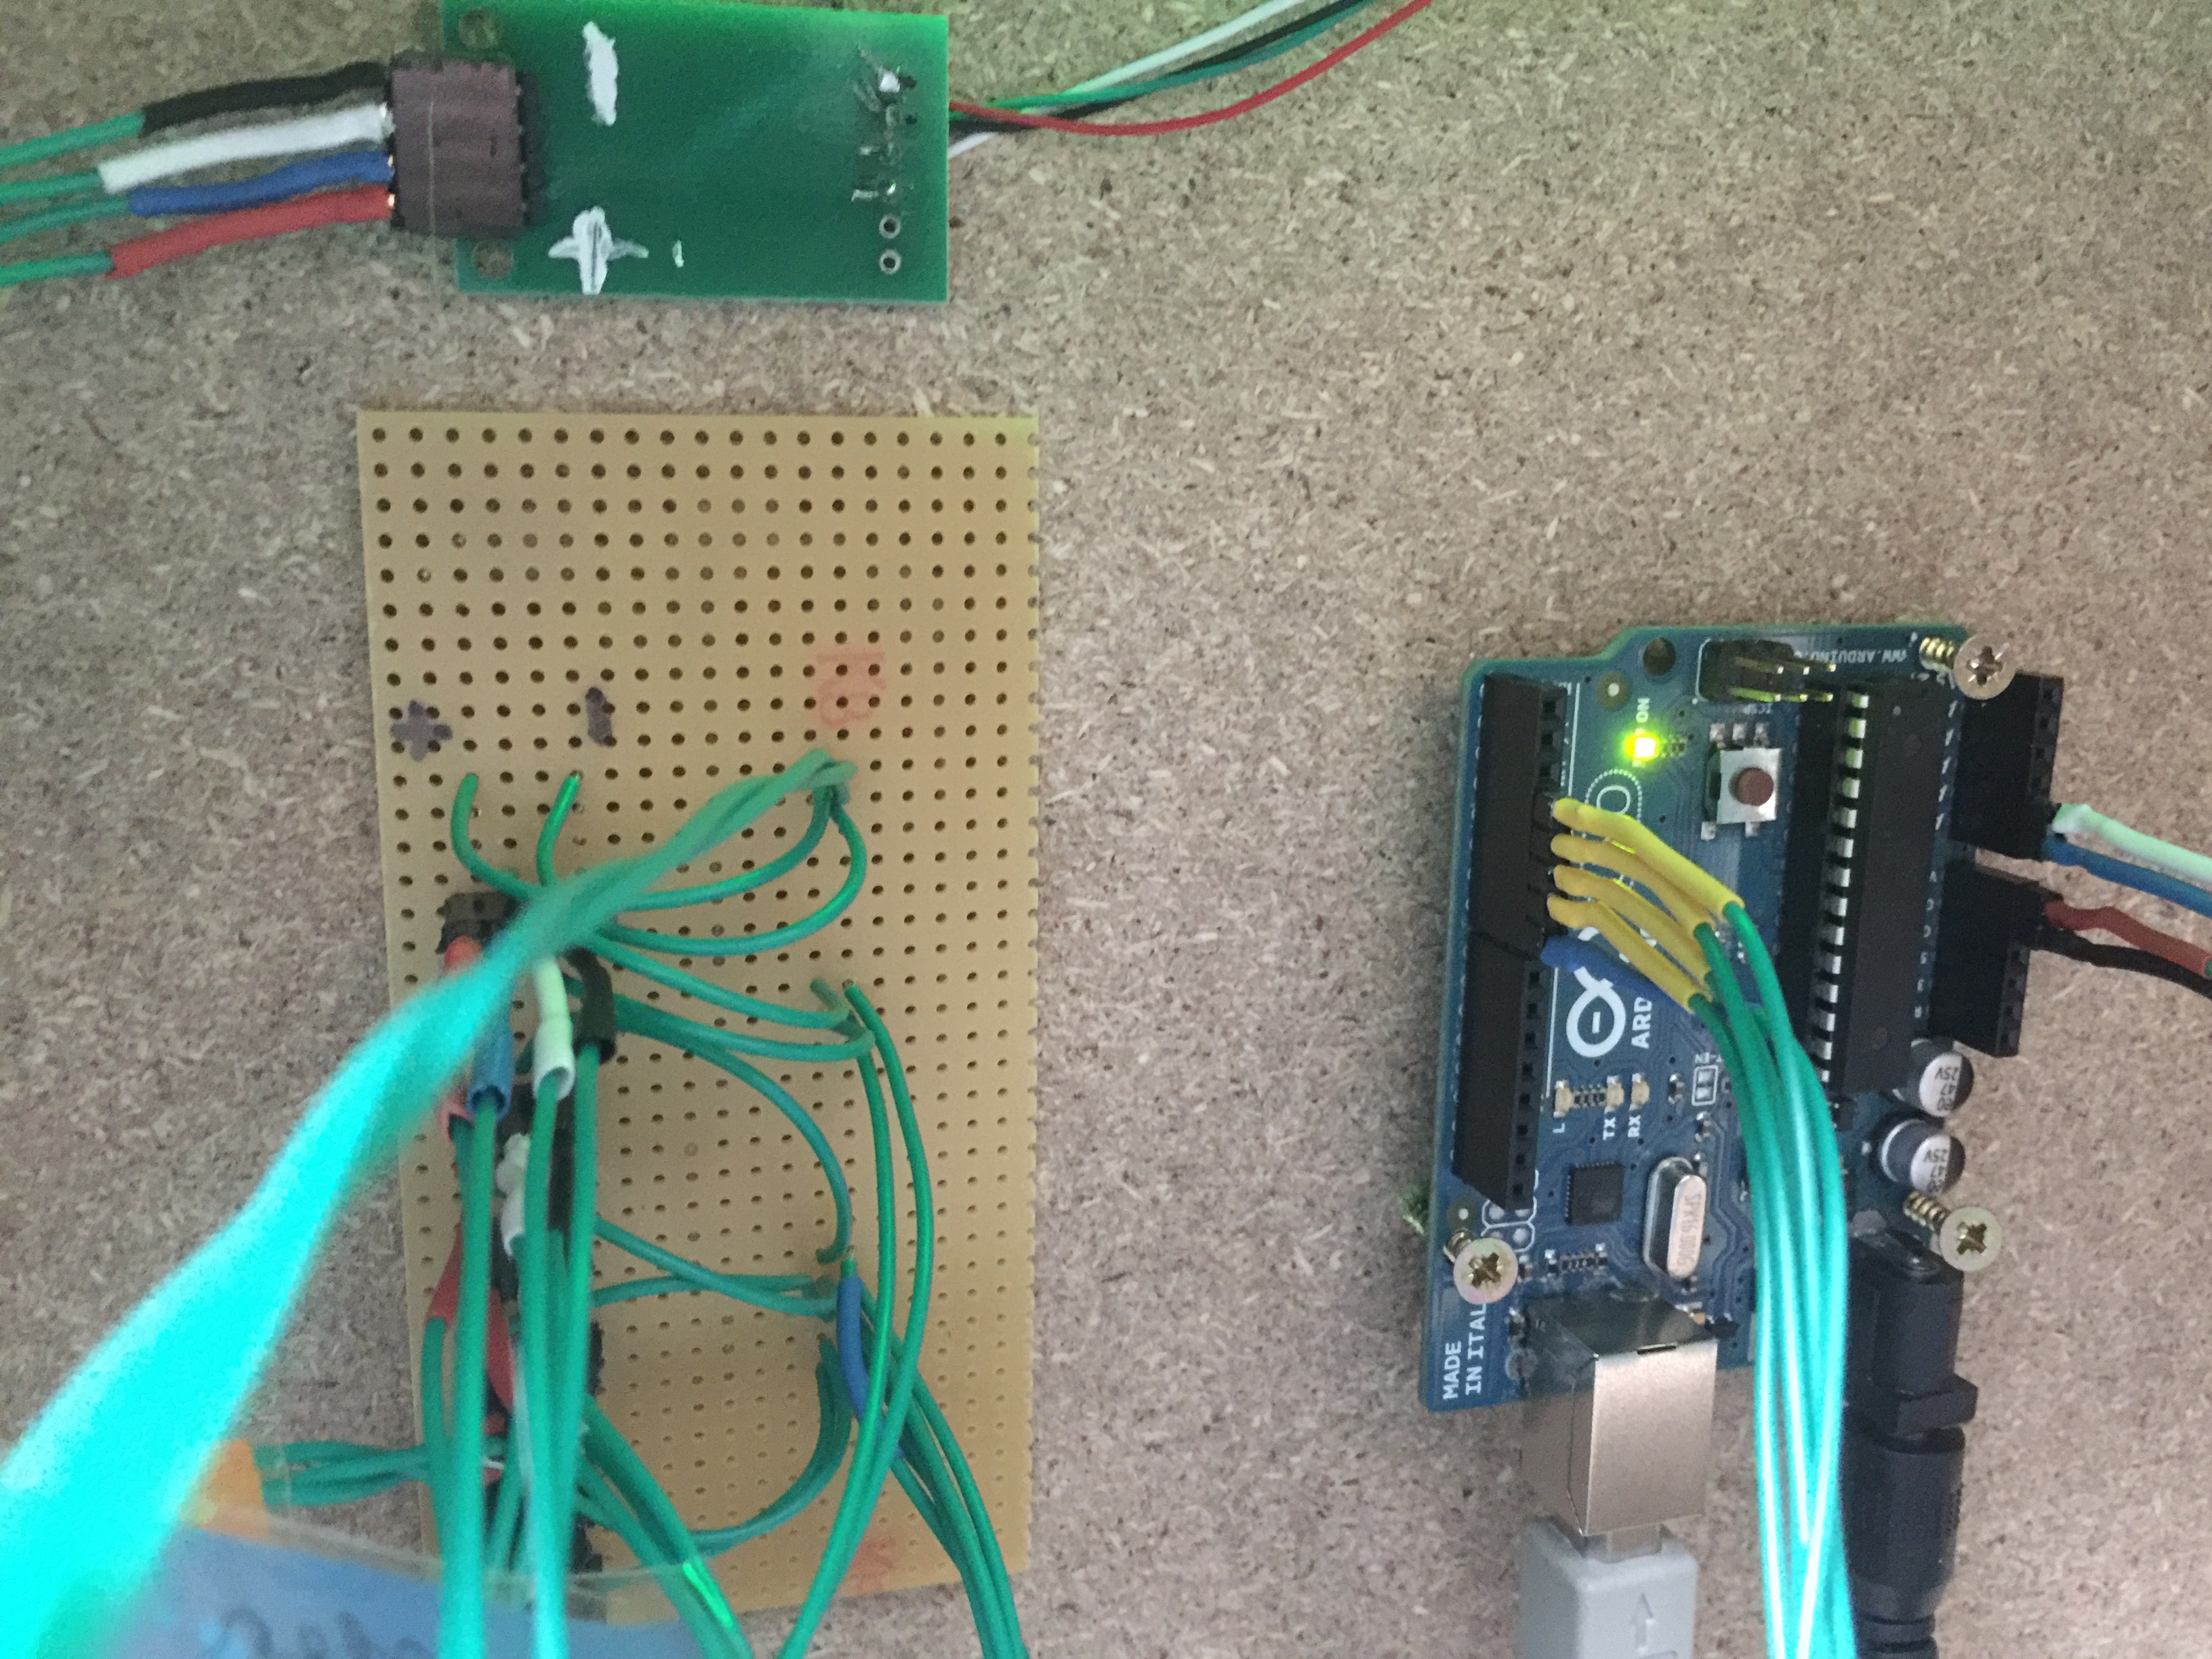
\includegraphics[width=0.8\linewidth]{pictures/built_in_electronic.JPG}}
\captionof{figure}{View from below: On the top left is the weighting module. On the bottom left is the circuit board where all LED stripes and the weighting module are connected to and which connects to the Arduino on the right}\label{fig:viewfrombelow}%      only if needed  
\end{minipage}

\begin{minipage}{\linewidth}% to keep image and caption on one page
\makebox[\linewidth]{%        to center the image
     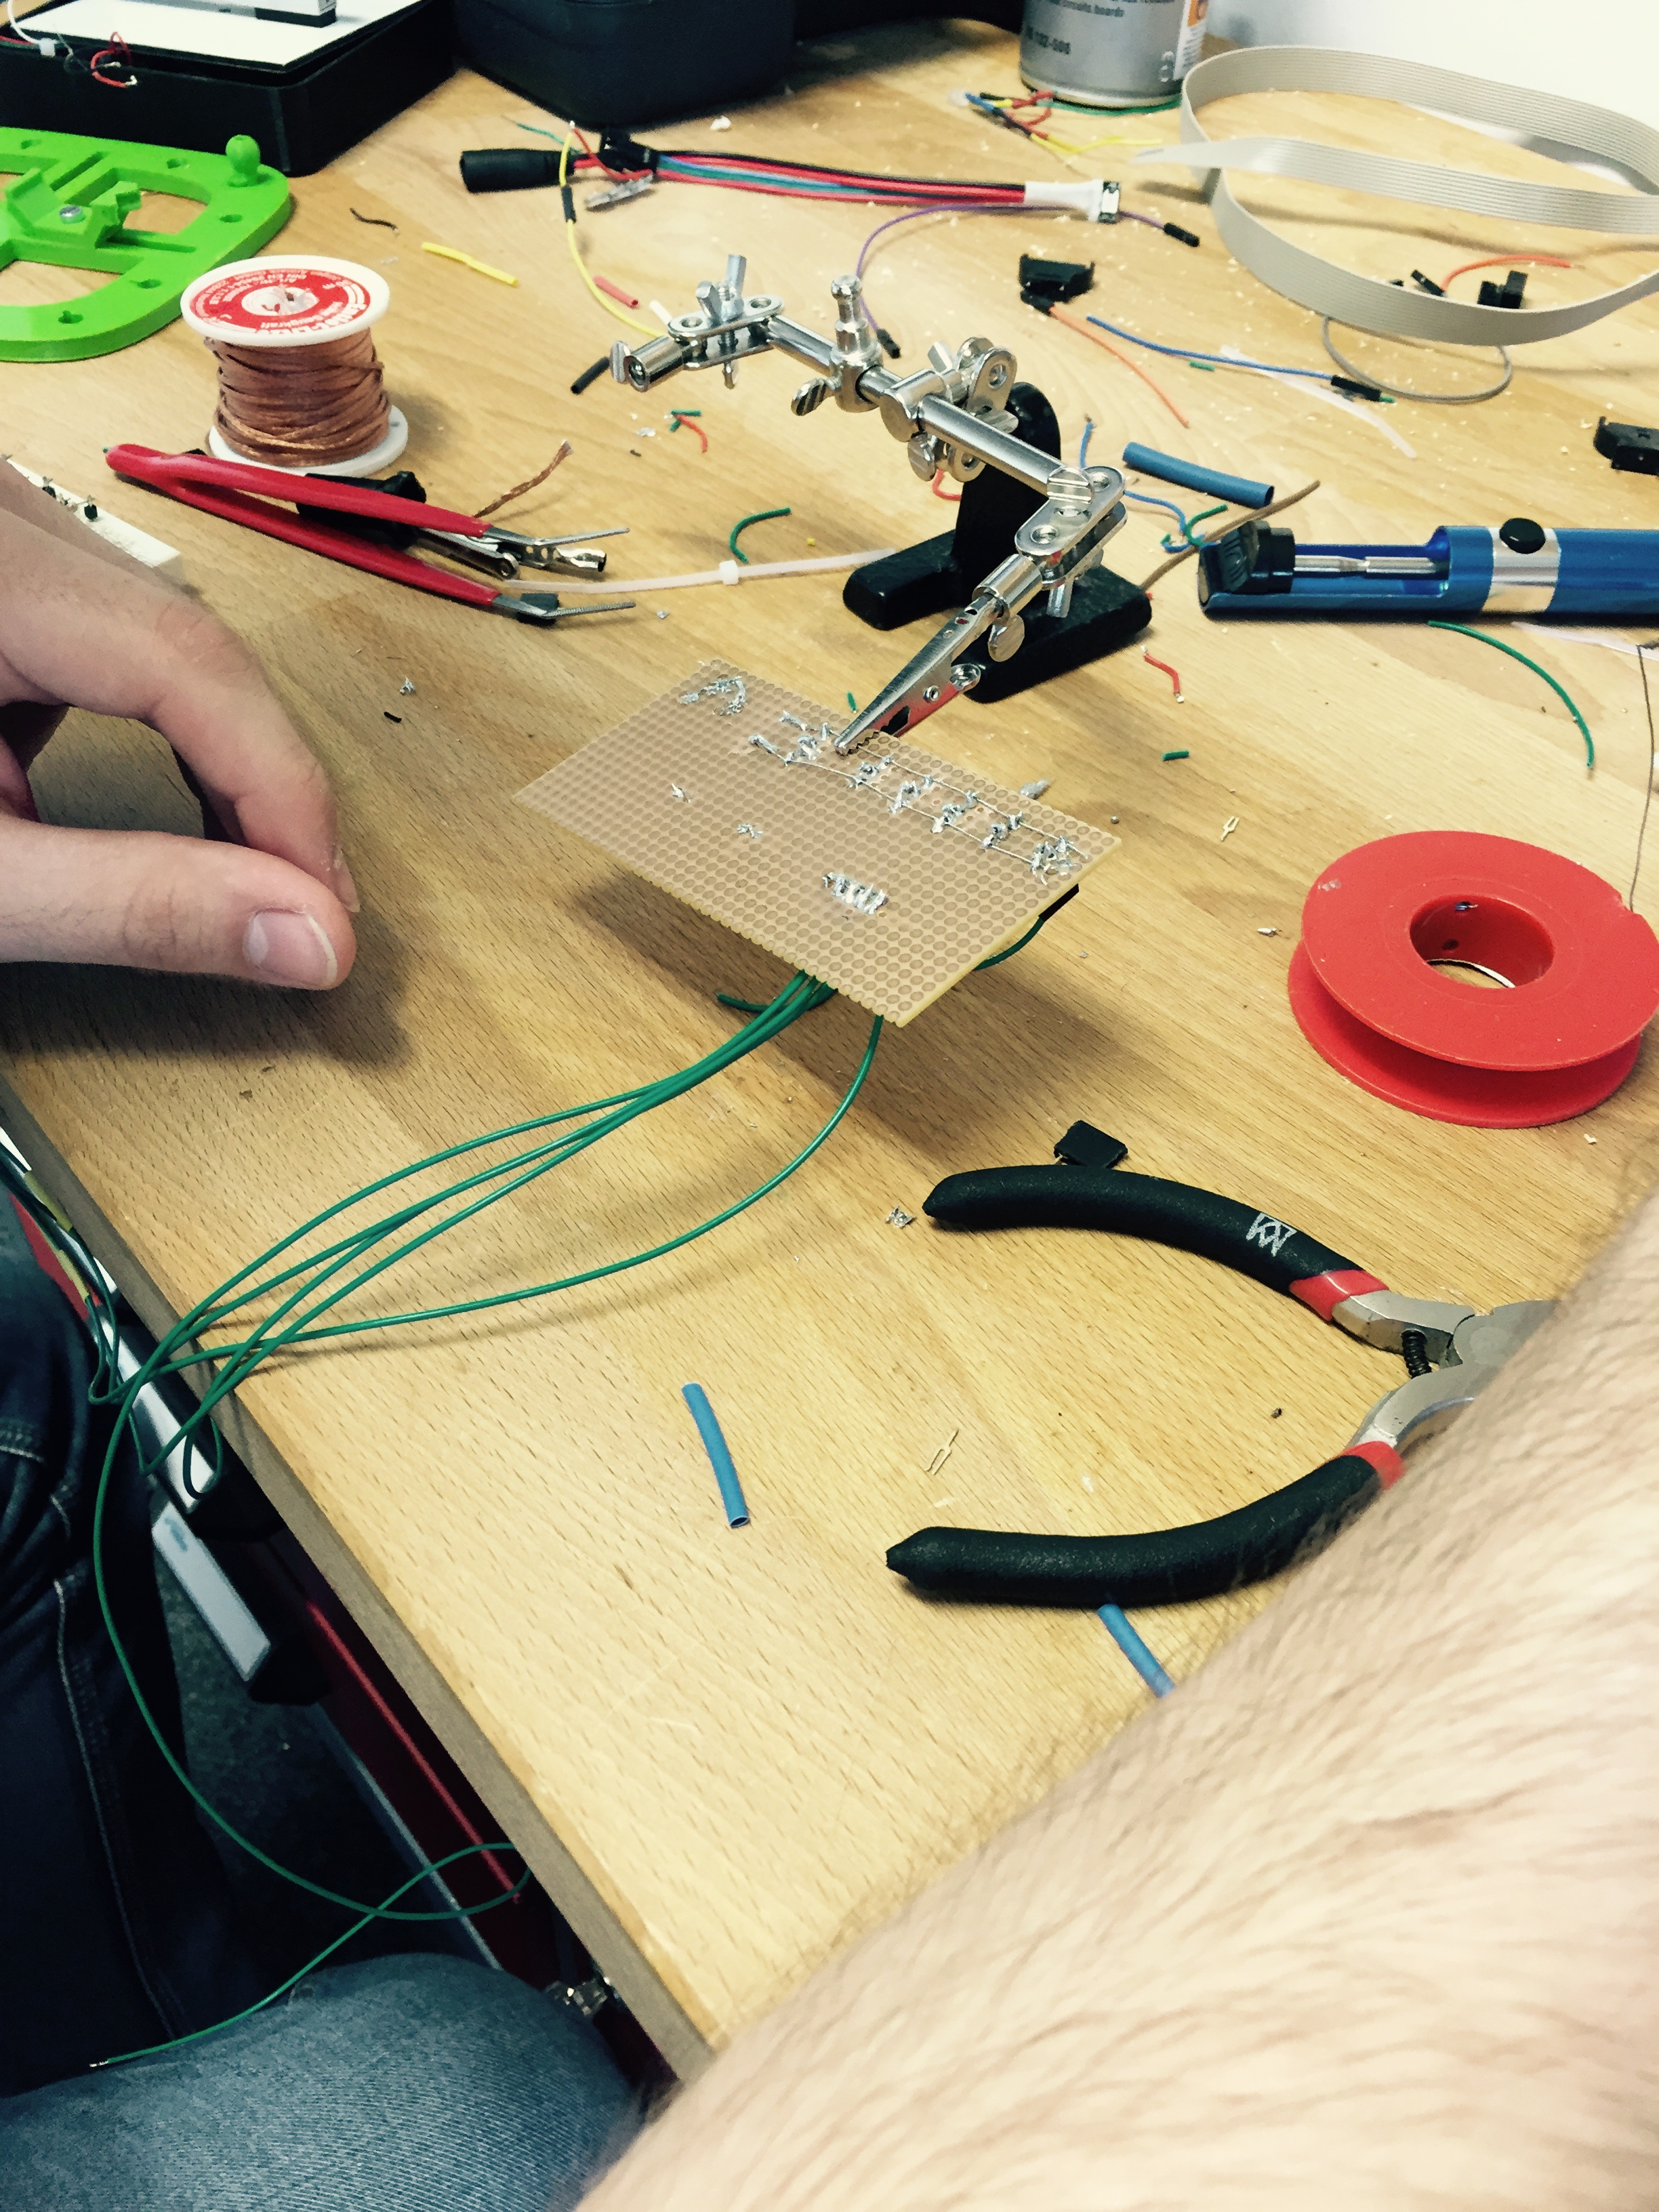
\includegraphics[width=0.7\linewidth]{pictures/wiring.jpg}}
\captionof{figure}{The circuit board during the soldering process}\label{fig:soldering}%      only if needed  
\end{minipage}



\section{Software Construction}
In this section the used electronic parts are described. Furthermore a illustration of the used software parts like the web server, user interface, database and the communication between the raspberry pi and arduino is given.

\subsection{Raspberry Pi and Arduino}
We use a Raspberry Pi 2 Model B. We installed raspian as the OS and enabled ssh so we can remote connect. We connected a WiFi-USB-dongle and setup a DHCP server and a network called \textit{CocktailPi} so users can connect to the bar. The Raspberry Pi is connected to a touch screen display, which we use to display the current step (see figure \ref{fig:rasp_arduino}, left).

The Arduino is an Arduino Uno rev3 (see figure \ref{fig:rasp_arduino}, right). It's a micro controller board with an 16Mhz processor and 32KB flash memory. It has 14 digital I/O and 6 analog input pins. The latter is also the reason why we need the Arduino, as the weighting module has 2 analog outputs and the Raspberry Pi has no analog inputs.

\begin{minipage}{\linewidth}% to keep image and caption on one page
\makebox[\linewidth]{%        to center the image
   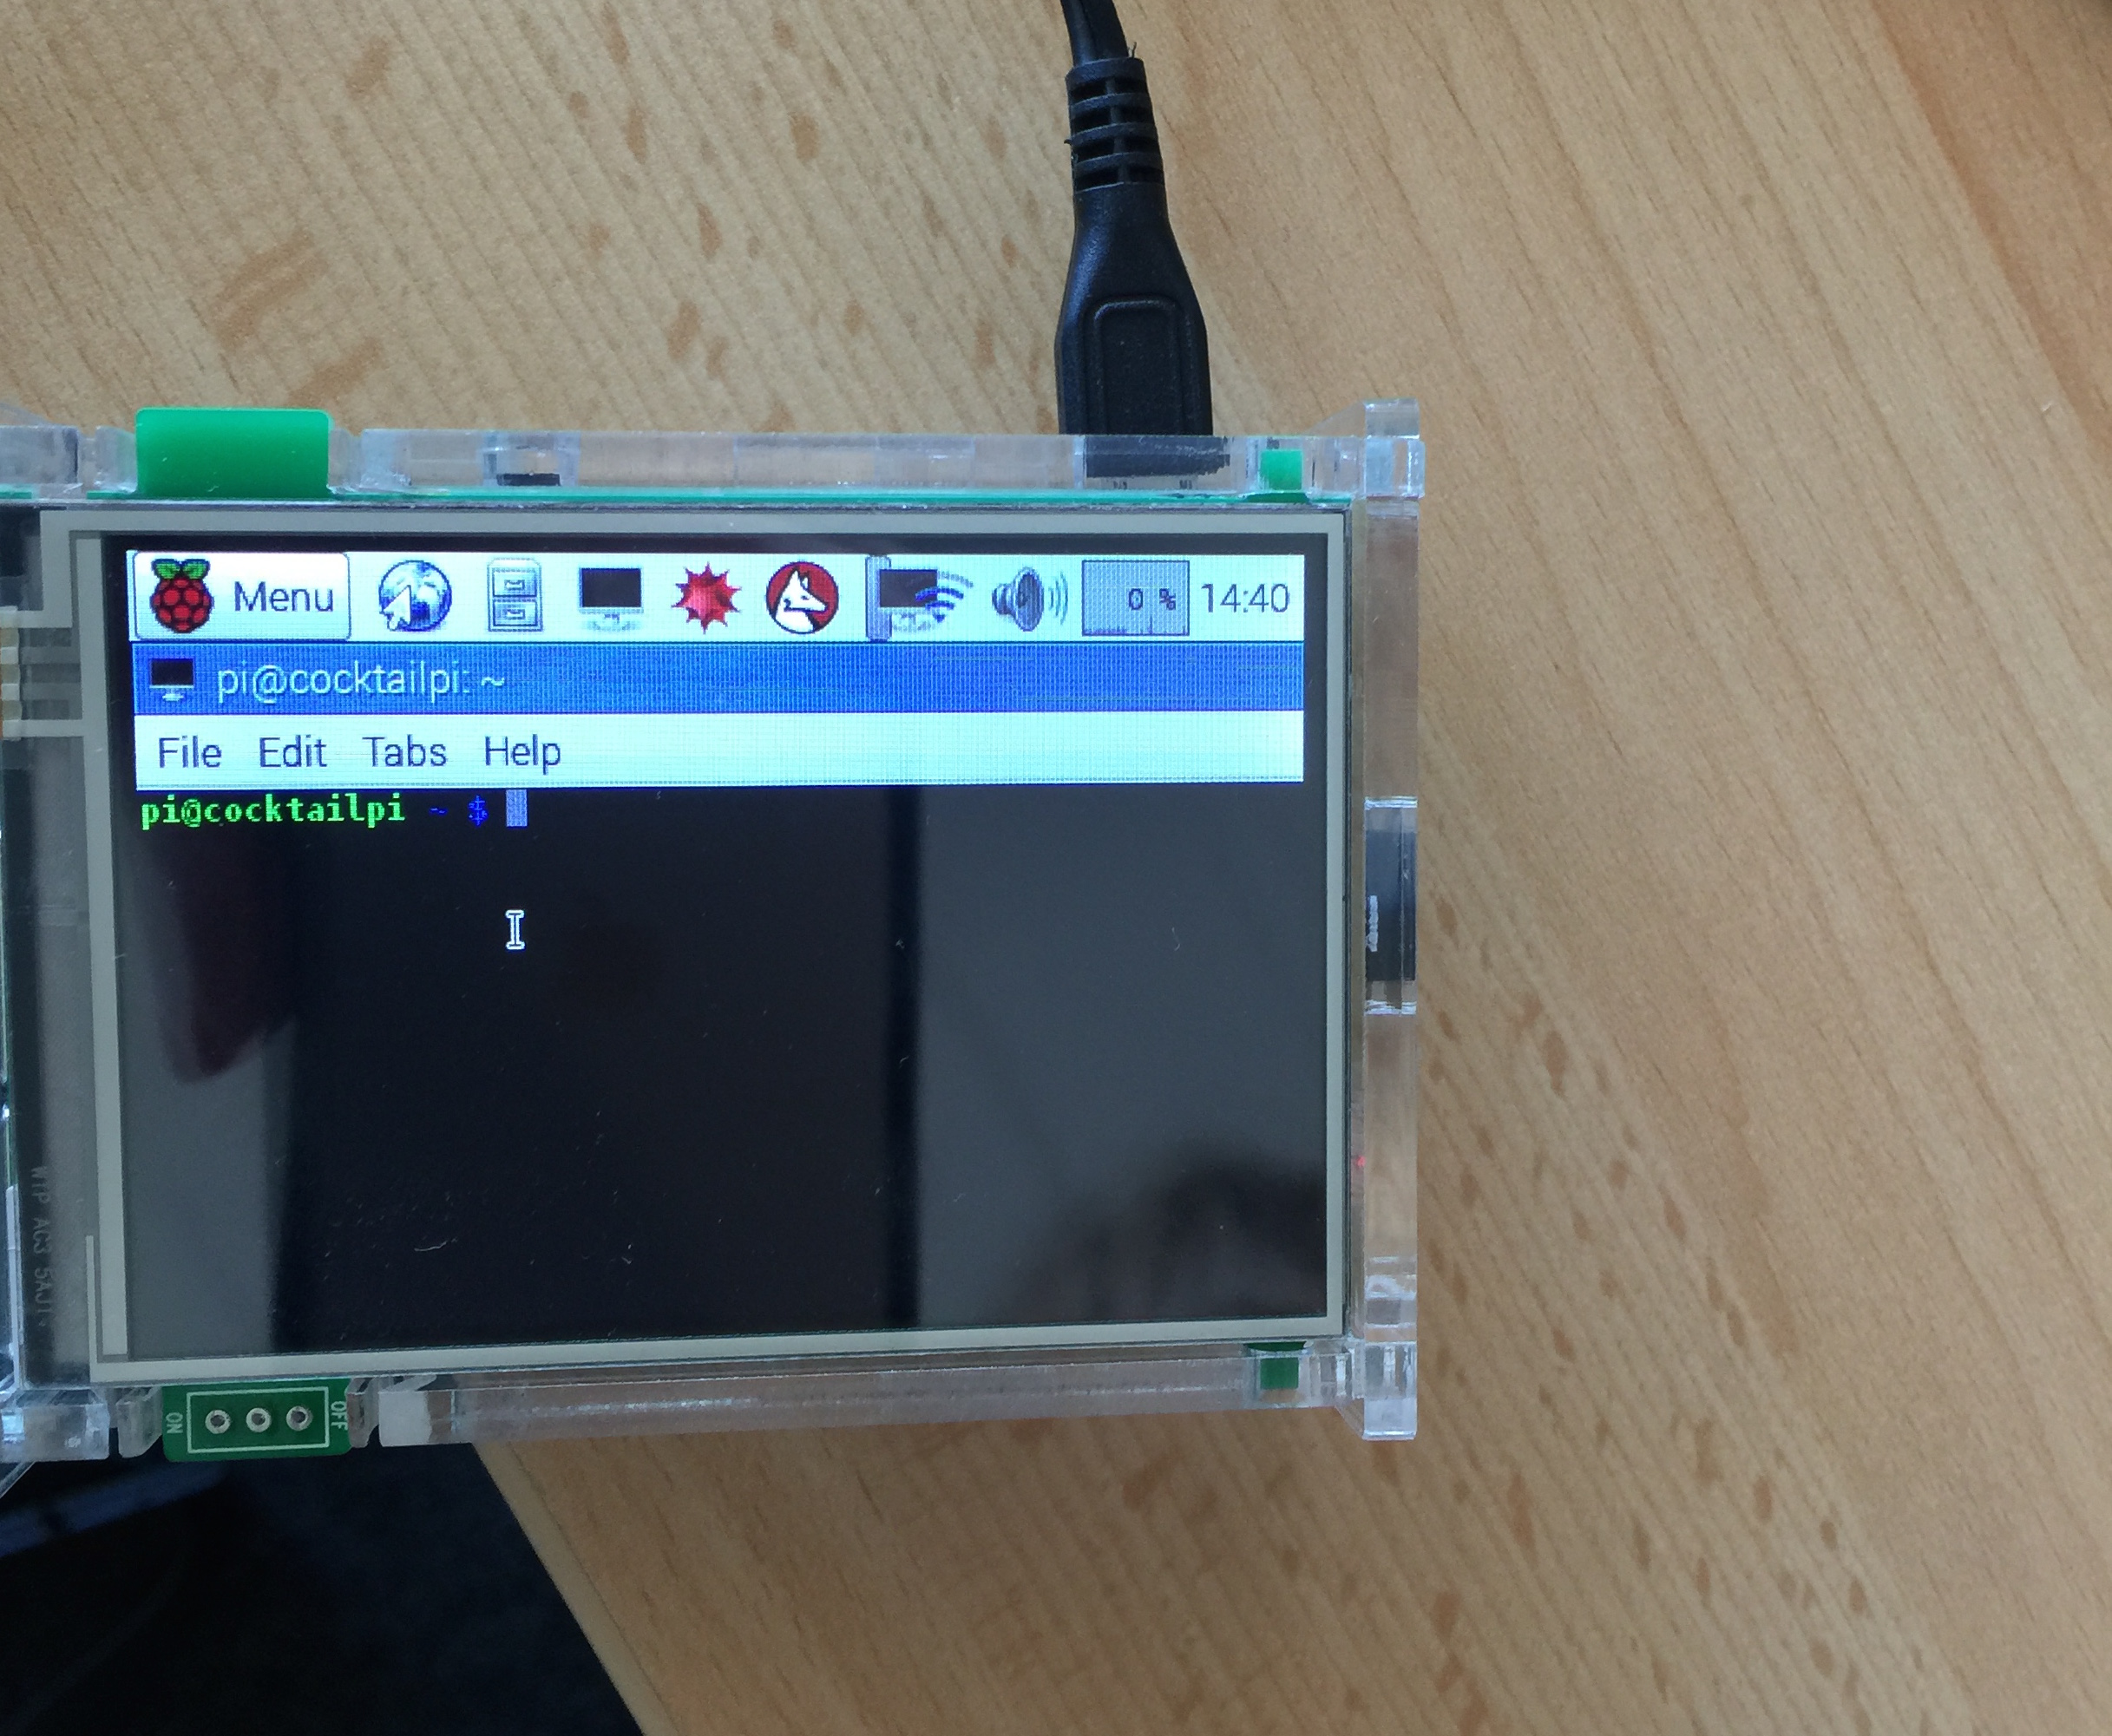
\includegraphics[width=0.5\linewidth]{pictures/raspberry_terminal.jpg}
   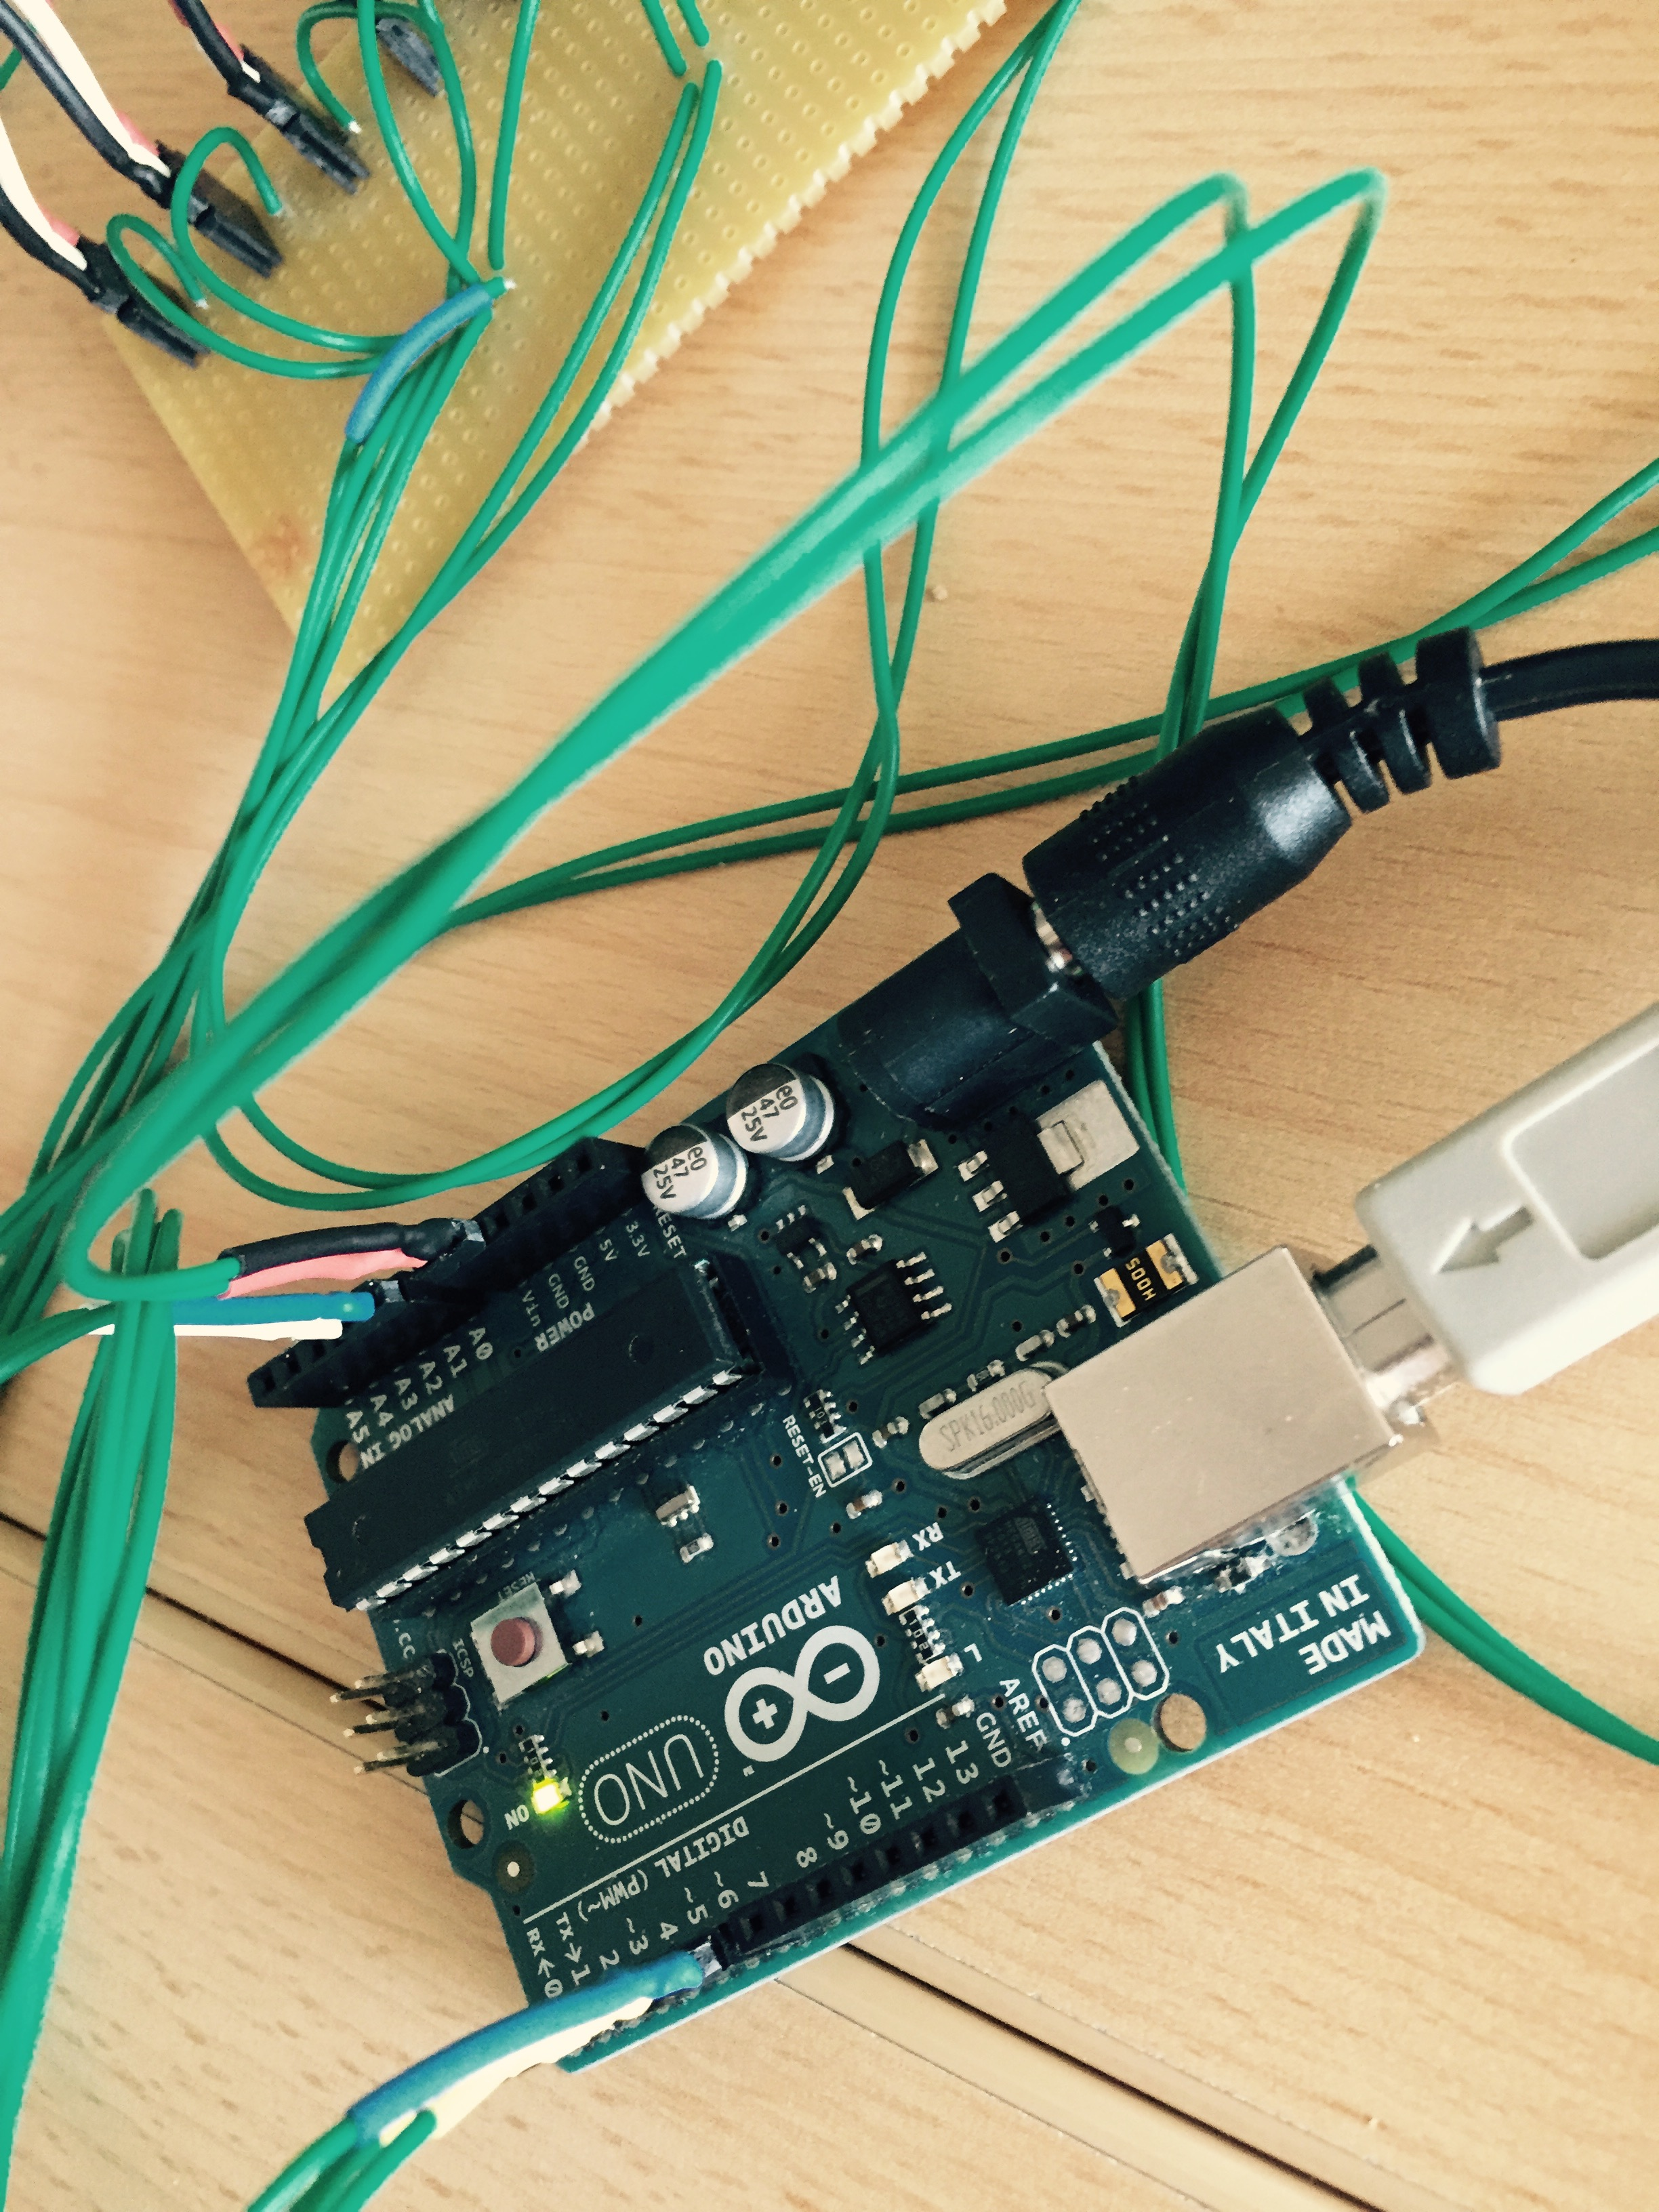
\includegraphics[width=0.5\linewidth]{pictures/arduino_mit_kabel2.jpg}}
\captionof{figure}{Left: Raspberry Pi with touch screen. Right: Arduino}\label{fig:rasp_arduino}%      only if needed  
\end{minipage}
 
\subsection{User Interface}
The user interface that is implemented for the system is designed as a web page. We based our interface on the free Bootstrap admin template "Metro". The interface provides the ability to view and filter all possible cocktails that can be mixed using "Bar Dude". Additionally information about the cocktails are displayed: cocktails are classified into four groups 'virgin', 'softy', 'pimp' and 'dude' consecutively ordered on their amount of alcohol. Furthermore information about the availability is displayed. The availability status is computed out of the availability of the different ingredients. \\
A button in each cocktail box is displayed and can be clicked to order the corresponding cocktail.

\subsection{Web server}\label{sec:web server}
We use \textit{Apache} as web server that will serve the static content of the page, scripts and images. Via \textit{mod\_wsgi} Apache connects to Django. mod\_wsgi is an Apache module that can run Python application which supports Python WSGI (Web Server Gateway Interface).

As Web Framework we use \textit{Django}. Django is Python based and uses a model/view/presenter schema. Django will receive the requested URL from Apache, then it will aggregate all information and data that are needed for the request and pass them to a HTML template, where the data is inserted and the final HTML is created, which Apache will serve to the user.



\subsection{Database}
We used internal Django interface to build the database. For development, we used SQLite3 and later on we switched to MySQL because SQLite3 cannot handle multiple accesses to the database. Since we use Django it is very easy to switch. All tables are saved as models and we only need to create the internal database. Django is also able to import the data from SQLite3 into MySQL. \\
To create tables in Django, models are used. A model declares the column names, the corresponding types and constrains. Then Django need to migrate the database with the following commands:
\begin{lstlisting}[language=bash]
 $ python manage.py makemigrations
 $ python manage.py migrate
\end{lstlisting}
While the server is running we can access '127.0.0.1/admin/' to enter entries into the created tables. We also could to this with normal SQL commands. Now we can select the table and add new entries (figure \ref{fig:db_entry}). \\
\begin{figure}[htbp] 
 \centering
    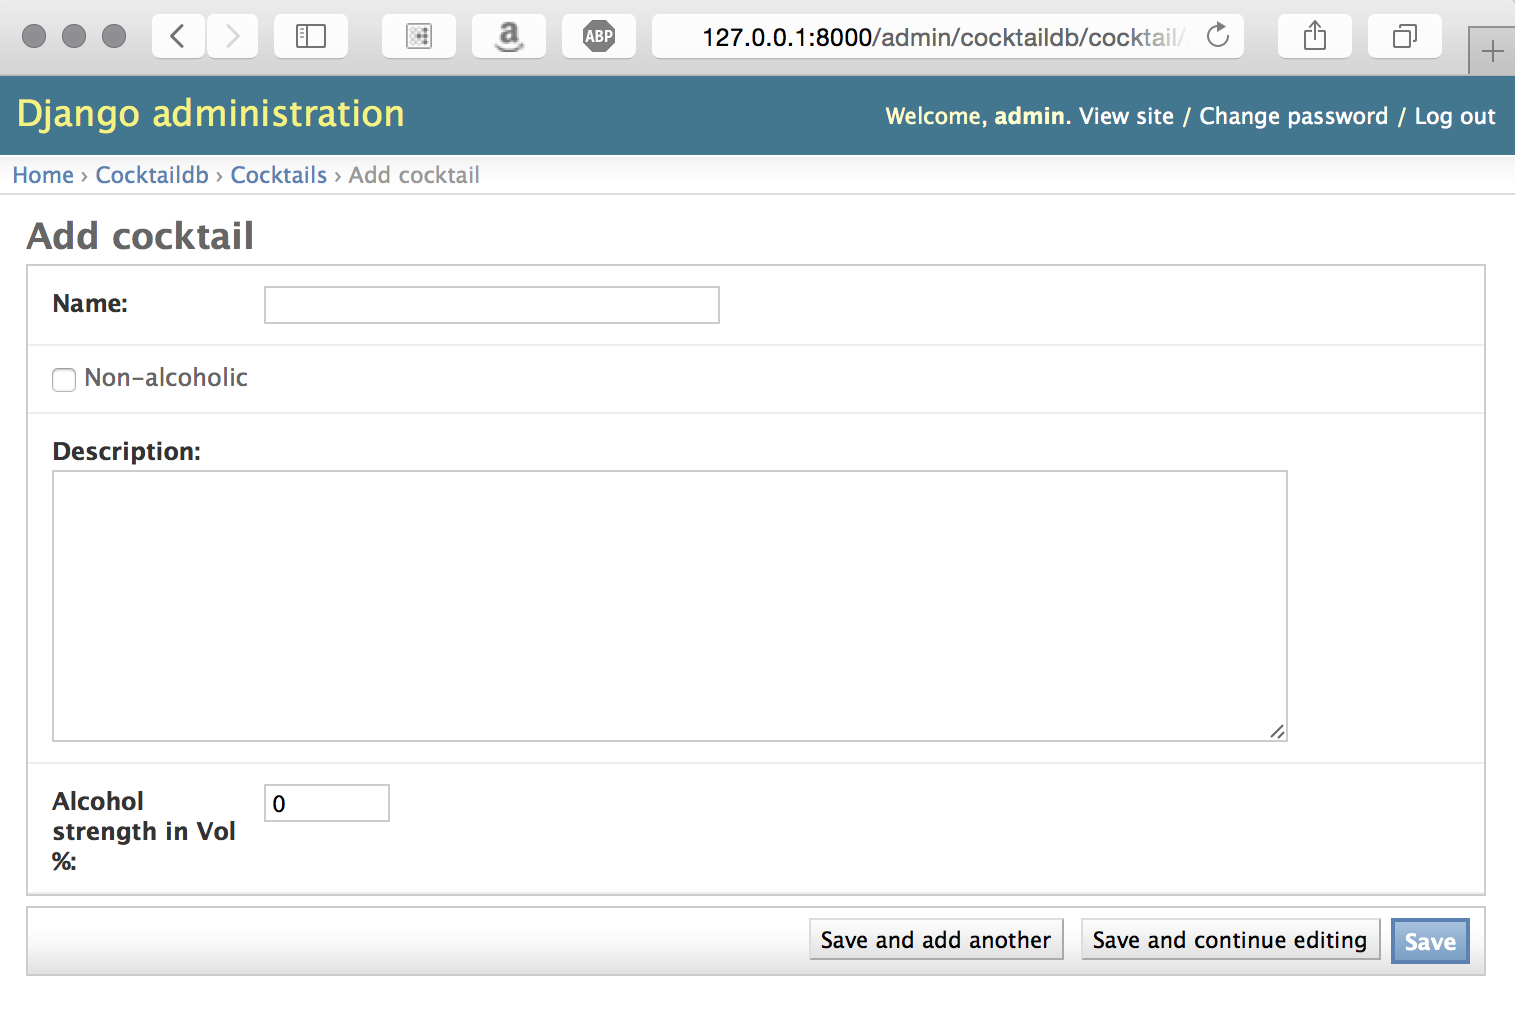
\includegraphics[width=0.8\linewidth]{pictures/db_insert_entry.png}
 \caption{Insert a new cocktail}
 \label{fig:db_entry}
\end{figure}
Django can handle all kinds of requests so that we do not need the normal SQL statements to ask for entries.

\subsection{Communication script}
To communicate between the Arduino and the Raspberry Pi we use a python script, which is started when the Raspberry Pi boots. It connects to the database and to the Arduino. We used a sym link to have a fixed name to connect to the Arduino. It also opens the browser. \\
The script runs as long as the Raspberry Pi is not shut down. It waits for input from the database in form of a new cocktail order which is not done yet. In case we are in step 0, it sends a beginning message to the Arduino which waits for the first touch of the weight measuring module. Otherwise it selects the first step of the current cocktail from the database and translates the step into a command which the Arduino can understand. The command consists always of nine characters and the first three encode the action. The next three characters can be empty or encode the ingredient. The last three characters can also be empty or encode the amount of an ingredient. If we need some information about time for mixing, shaking or filling the content of the shaker into a glass, we send it in the last six characters. \\
The Arduino always send an answer which can either be the message it received, 'READY' if an action has finished, 'TOUCHED' if someone touched the weight measuring module to start the process, 'NO\_INPUT' if no one touched the weight measuring module to start the process or 'ERROR' if the message lost some content. In case of an 'ERROR' message the message is sent again. In case of an 'NO\_INPUT' message the current order is deleted in the database.

\subsection{Communication protocol}
We developed a simple numbers based communication protocol between the Raspberry Pi and the Arduino. After starting the Arduino it waits for a message consisting of 9 characters. If the size is incorrect it will respond with \textit{ERRROR} to the Raspberry. If the message has the correct length it will first send back the received message for checking by the Arduino and then execute the command that was encoded in the message. The first 3 characters denote the mode that will be chosen, by converting the characters one by one to a number until a non numeric character appears. In the following we denote non numeric characters with a \texttt{.} Possible commands are:

\begin{itemize}
\item \texttt{0.. ... ...} switches all lights off.
\item \texttt{1.. ... ...} enables the so called \textit{party mode} until an other command arrives
\item \texttt{2.. ppp www} enables the \textit{whole weight measuring mode}, where position $ p $ will be illuminated until the scale has the weight $w$ grams and then sends \textit{READY} to the Raspberry Pi. \textit{This was used for debugging purposes only.}
\item \texttt{3.. ppp www} enables the \textit{added weight measuring mode}, where position $ p $ will be illuminated until  $w$ grams have been added to the weight that is measured when issuing the command and then sends \textit{READY} to the Raspberry Pi.
\item \texttt{4.. ... ...} returns the current weight in grams over the serial connection. \textit{This was used for debugging purposes only.}
\item \texttt{5.. ... ...} illuminates the glasses until one is placed on the scale and then sends \textit{READY} to the Raspberry Pi.
\item \texttt{6.. ... ...} illuminates the shaker until it is placed on the scale and then sends \textit{READY} to the Raspberry Pi.
\item \texttt{7.. ... ...} illuminates the glasses and waits until one is taken, placed on the scale and filled with the content of the shaker and then sends \textit{READY} to the Raspberry Pi.
\item \texttt{8.. ttt ttt} illuminates the bar  for $t$ milliseconds in a way that inspires the user to shake the shaker, waits until the shaker is placed on the scale again and then sends \textit{READY} to the Raspberry Pi. 
\item \texttt{9.. ttt ttt} illuminates the bar for $t$ milliseconds in a way that inspires the user to stir his drink with a spoon and then sends \textit{READY} to the Raspberry Pi.
\item \texttt{11. ttt ttt} waits for $t$ milliseconds that the user touches the scale. If the user touched the scale the Arduino sends {TOUCHED} to the Raspberry Pi, else it will send \textit{NO\_INPUT}.
\item \texttt{12. ... ...} measures the current weight and will display the \textit{party mode} until the weight from the scale is removed.

\end{itemize}

Any other command number will trigger the \textit{error mode}, which causes the whole bar to blink in red.

\section{User Guide}
In this section a overview of how to use the system is given.
\subsection{Start the System}
To start the system you just need to connect the bar to the power supply system. After that the Raspberry Pi boots and when the 'Bar Dude' website is displayed, you can start ordering your cocktails. \\
To initialize the system you have to enter the current amount of each ingredient. After connecting to 'CocktailPi' described in the next subsection go to '192.168.0.1/admin/' and log in with 'admin' and 'ubercocktail'. Then select 'Ingredients' and edit the amount. You also should do this when you replace a bottle.
 \subsection{Select a Cocktail}
You have to connect to the Access Point 'CocktailPi' and log in with the password 'CocktailPi'. Then go to '192.168.0.1' in your browser. Now you can see the interface where you can choose your cocktail, which you can see in figure \ref{fig:select_cocktail}. For more information about the website read section \ref{sec:web server}. You choose your cocktail by clicking on the corresponding 'Do it dude!' button. You get a number to know which cocktail is your's.

\begin{minipage}{\linewidth}% to keep image and caption on one page
\makebox[\linewidth]{%        to center the image
  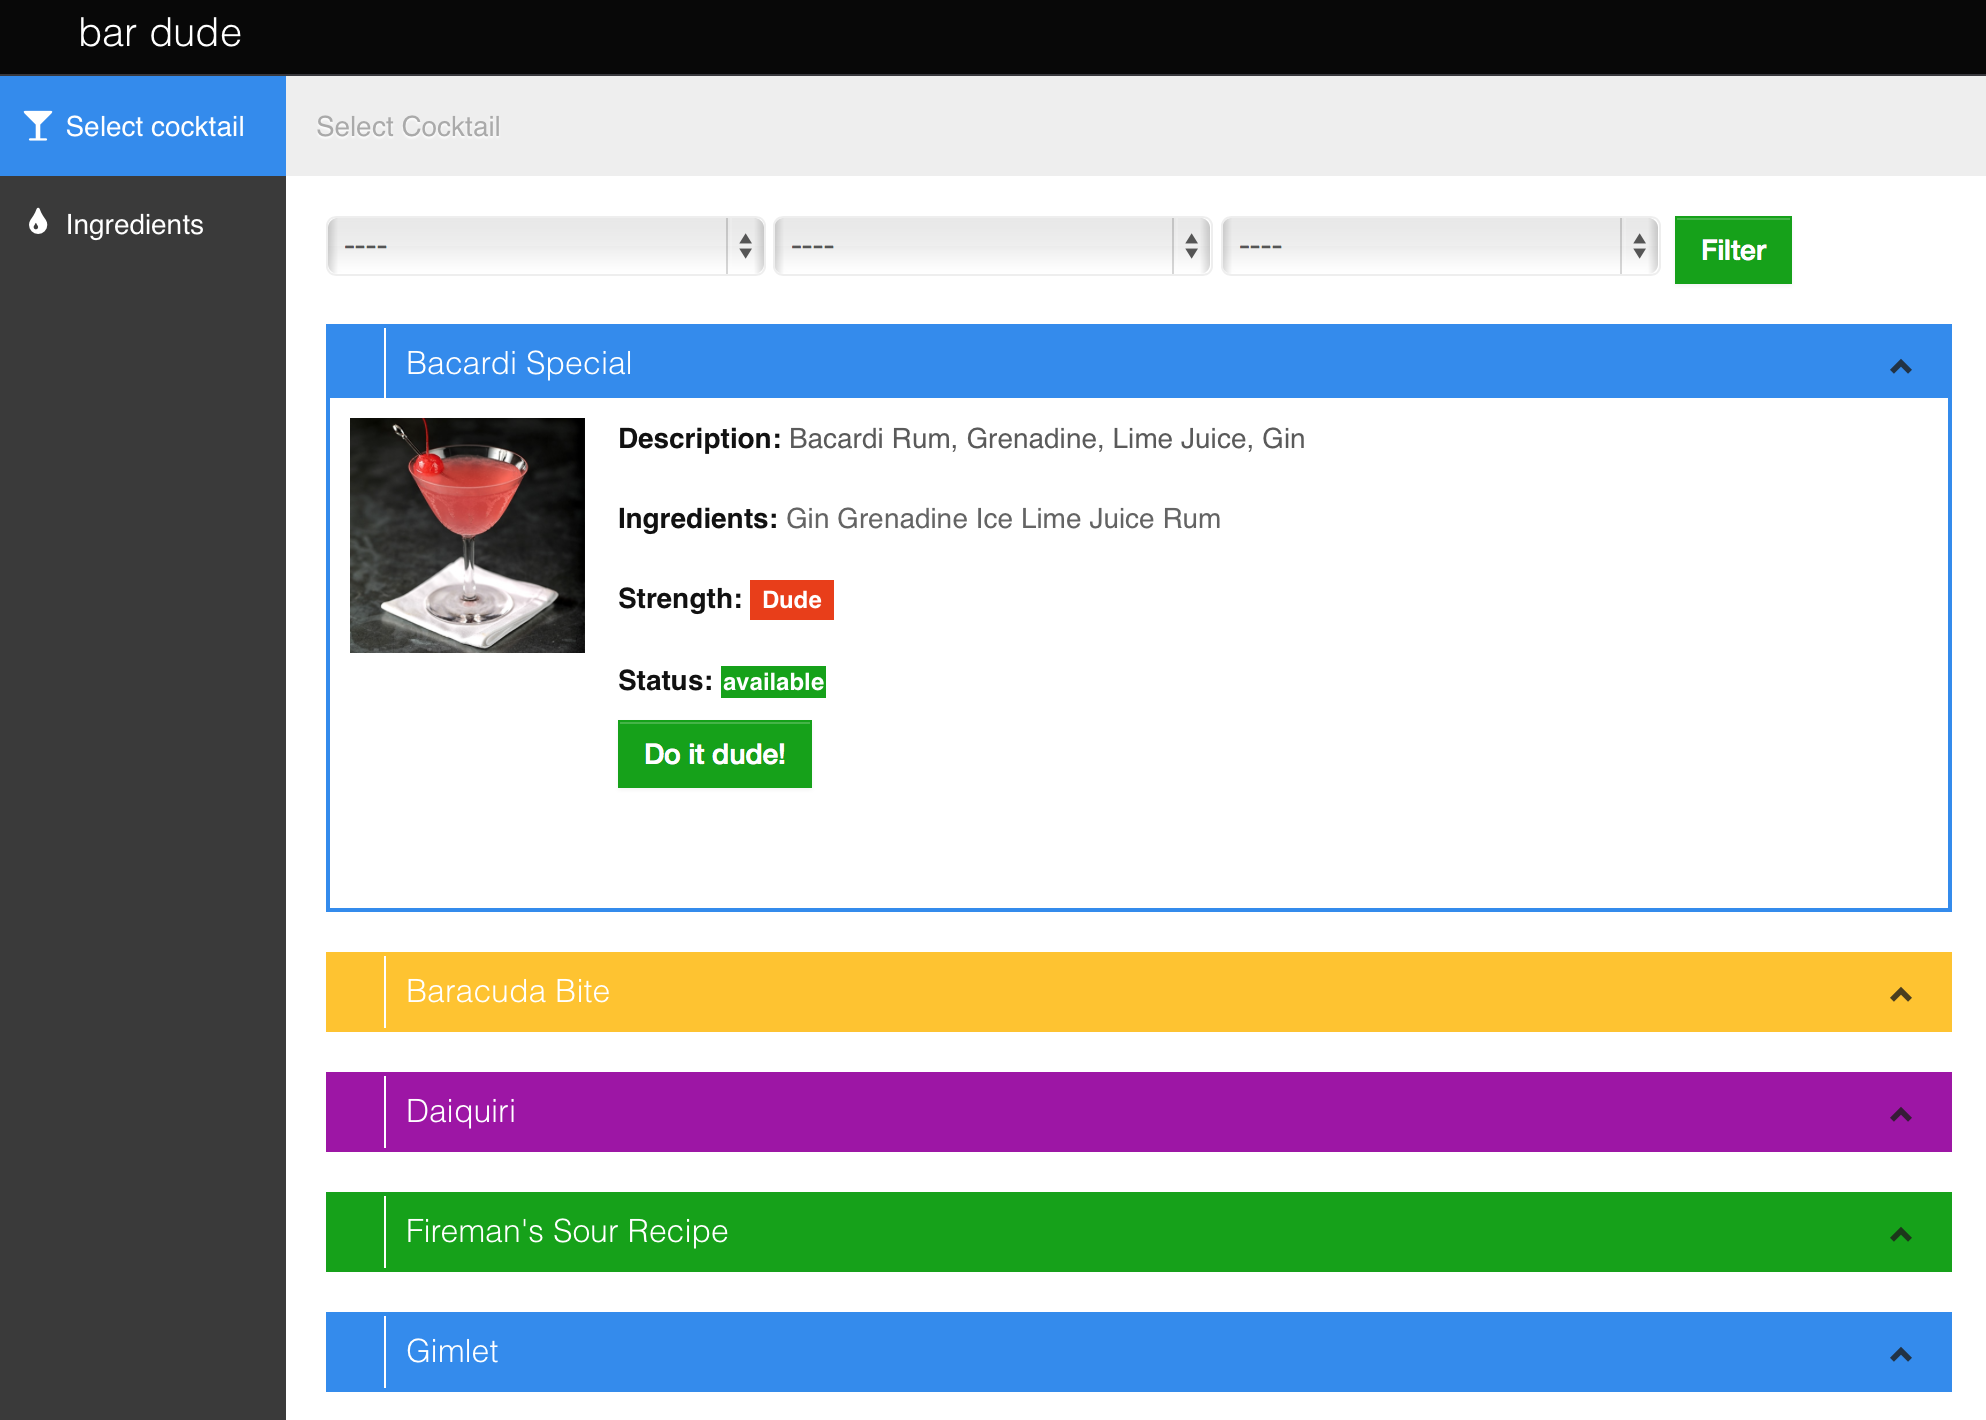
\includegraphics[width=0.8\linewidth]{pictures/select_cocktail.png}}
\captionof{figure}{Selection of a Cocktail}\label{fig:select_cocktail}%      only if needed  
\end{minipage}

 \subsection{Mix the Cocktail}
When your number is displayed on the display of the Raspberry Pi, you have 30 seconds to touch the weight measuring module. It also displays the countdown. If the time runs out, the order is deleted and the next cocktail number is displayed. 
\\

\begin{minipage}{\linewidth}% to keep image and caption on one page
\makebox[\linewidth]{%        to center the image
   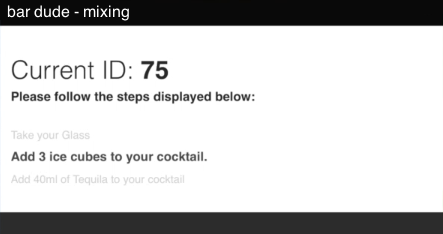
\includegraphics[width=0.8\linewidth]{pictures/raspberry_mixing.png}}
\captionof{figure}{The surface of the Raspberry Pi during the mixing of the cocktail\\}\label{fig:raspberry_mixing}%      only if needed  
\end{minipage}
Now you can follow the instructions of the display, as shown in figure \ref{fig:raspberry_mixing}. First you have to take a glass or a shaker depending on which is illuminated and put it on the weight measuring module. Then you add the illuminated ingredients. The weight measuring module shows you which amount of the ingredient is needed. It changes the color from red to green and the speed of the illumination slows down until you fill in enough. If you use a shaker you have to shake it when the bar goes wild. Then you have to take a glass and fill the content of the shaker into the glass. If you take a glass at first, you normally, not always, have to mix your cocktail. In this case the weight measuring module displays a circle. Take a spoon and mix until the next step is displayed. When your cocktail is finished, a party mode is displayed. 


\section{Conclusions}
We built a system called ``Bar Dude" (figure \ref{fig:bar}) that combines interactive lighting elements with affective computing to guide users of the system throughout the mixing procedure of an arbitrary cocktail. Whereby we fulfilled the requirements of the seminar ``Affective Lighting". \\
``Bar Dude" allows a user to select a cocktail out of a selection of circa 50 different ones via a provided web application. The system assigns an ID to the user and asks him to go to the bar. There he or she can follow the self explaining advices given via light signals, such that a user with no prior knowledge of bartending can mix a cocktail. \\
In our first field tests ``Bar Dude" performed quite good. At a small to medium party or an event where an hired bartender is not affordable, but one nevertheless wants to serve cocktails to his guests, ``Bar Dude" is a good and keen alternative.

\begin{minipage}{\linewidth}% to keep image and caption on one page
\makebox[\linewidth]{%        to center the image
   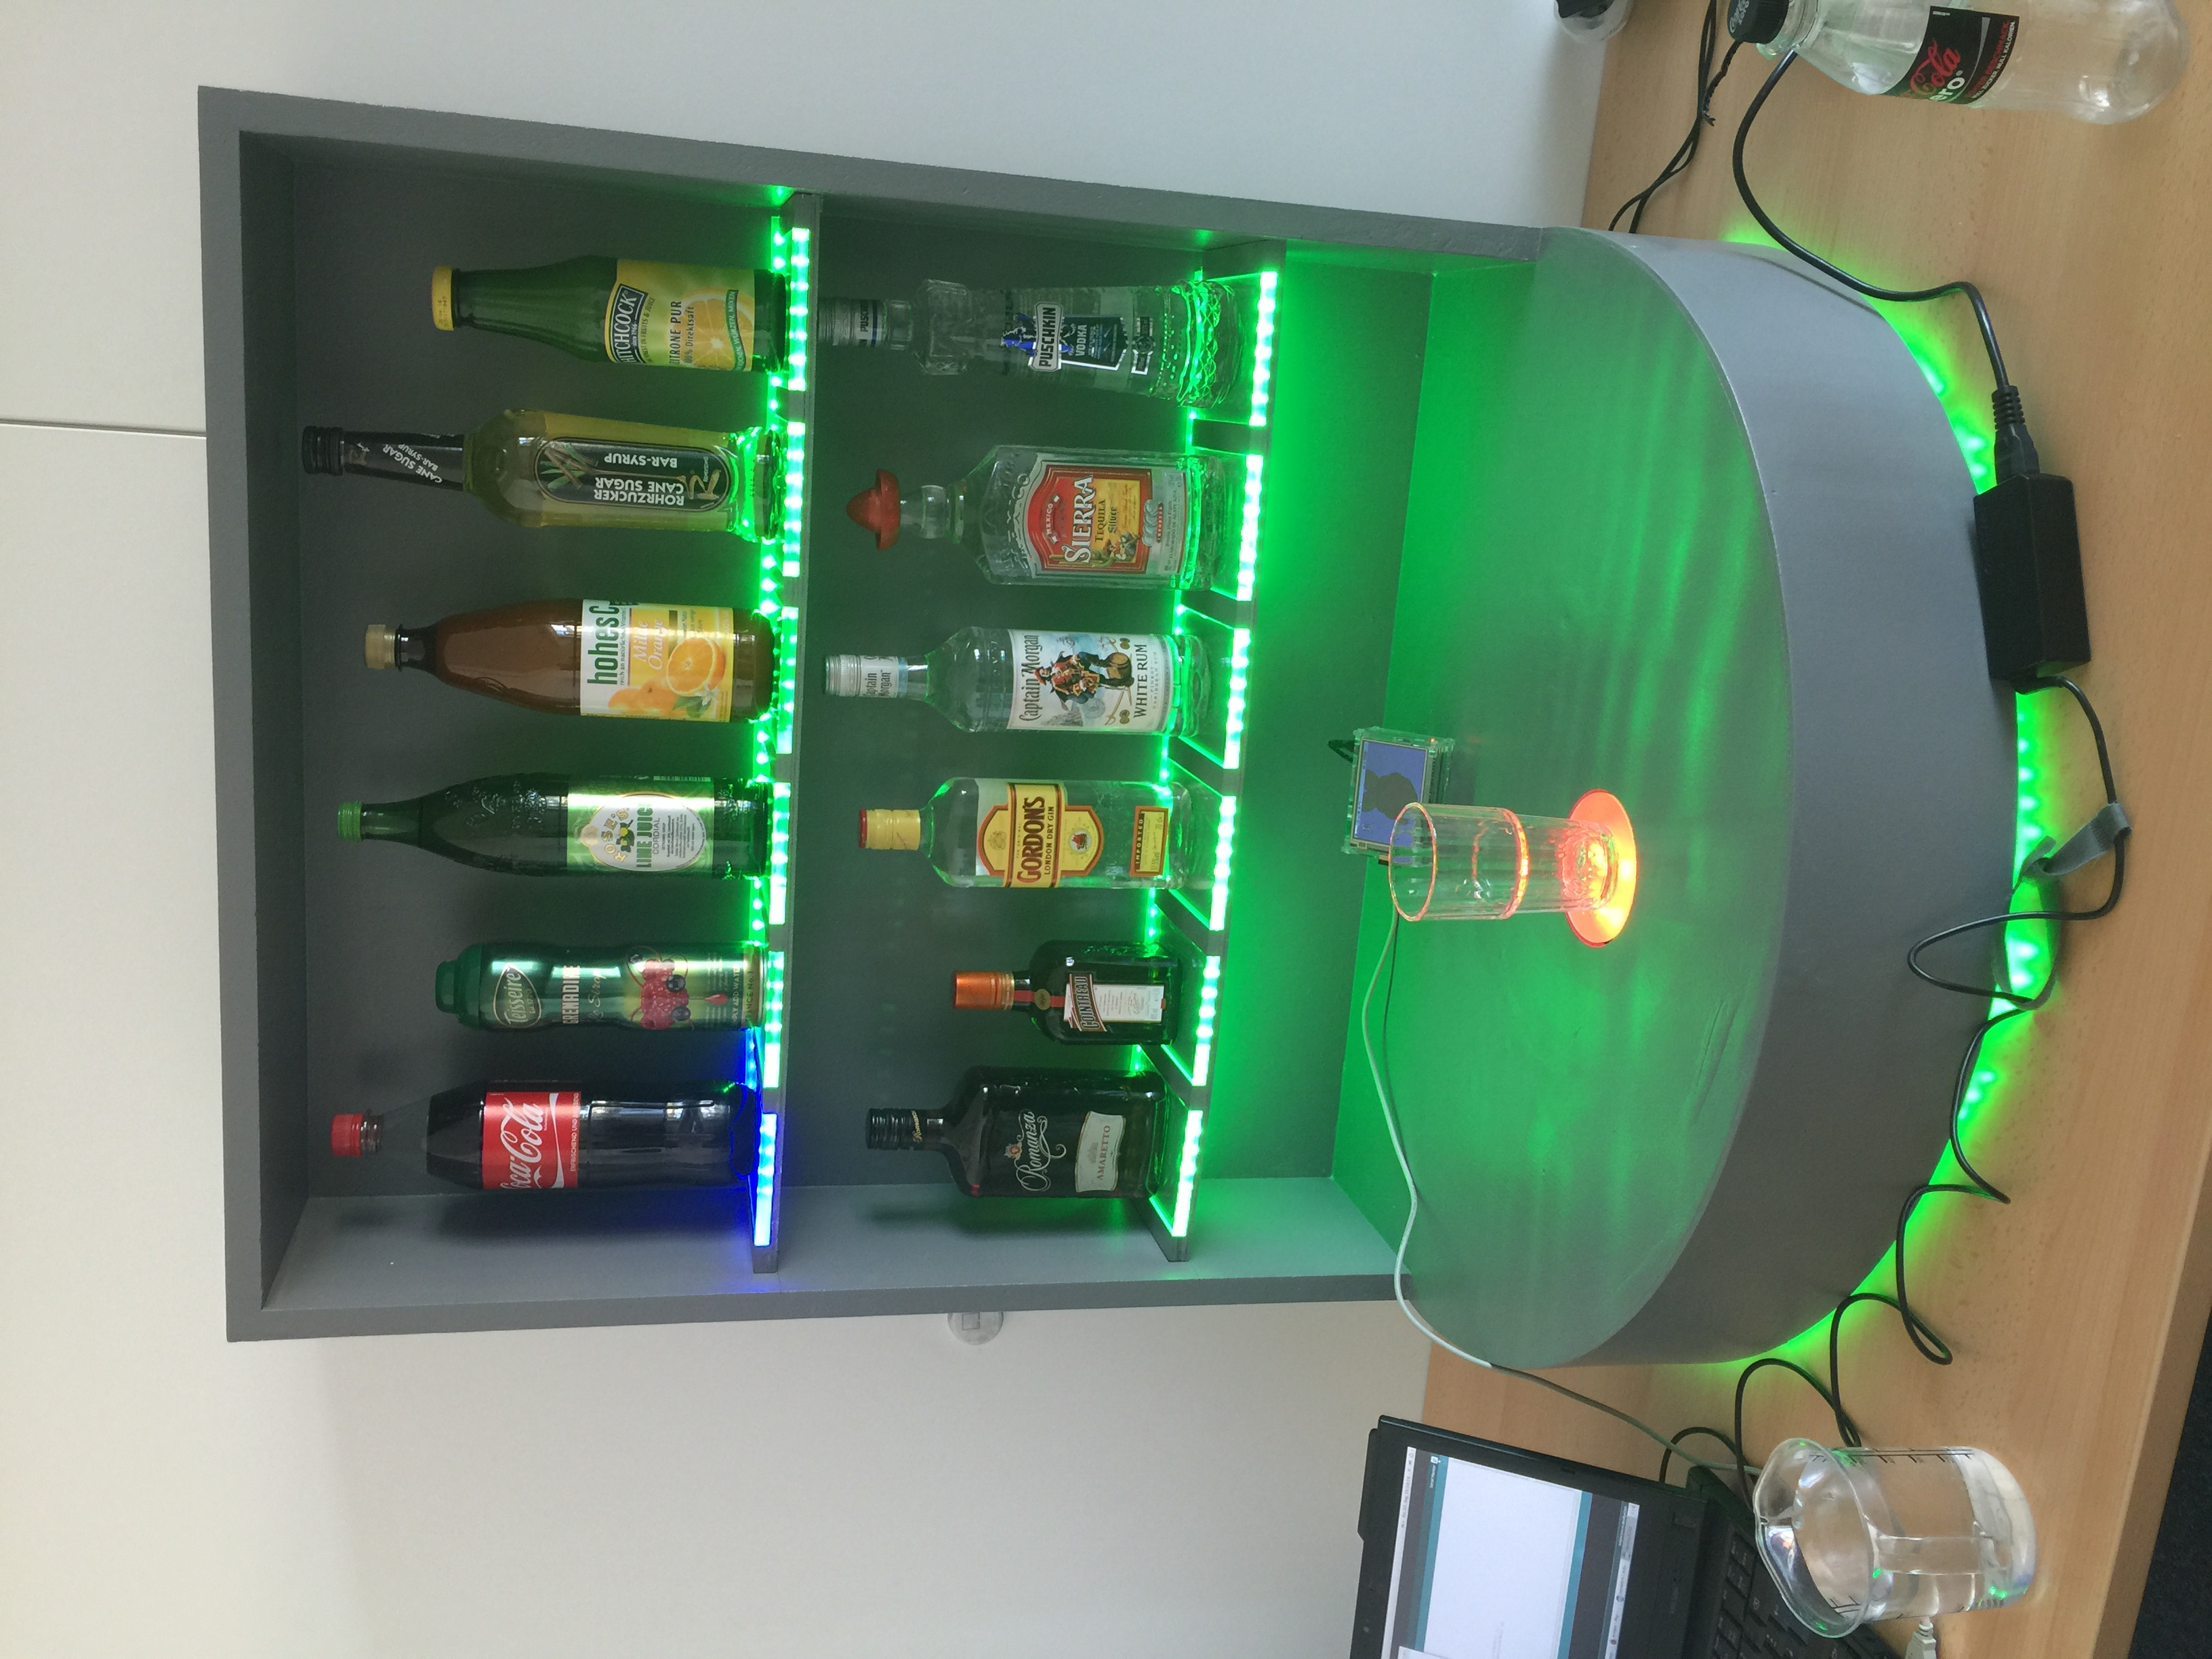
\includegraphics[width=0.8\linewidth, angle =270]{pictures/bar.jpg}}
\captionof{figure}{Finished bar}\label{fig:bar}%      only if needed  
\end{minipage}

\section{Future Work}
Apart from our initial idea the system could be extended to a bartender school. That means users can acquire knowledge of cocktail mixing by using ``Bar Dude" in its described form. Additionally an examination mode is implemented. One would have to extend the system with RFID readers and suitable RFID labels on the ingredients to locate them. So the system could determine which ingredient was taken from the shelves in which step. In the examination mode first a cocktail is selected in known manner, but all LEDs are turned off. A bartender apprentice is asked to mix a cocktail without visual assist from the system. If he or she selects the right ingredient in the very step the ingredient is lighted green, red otherwise. In this setting ``Bar Dude" could be more than just an assistance in cocktail mixing, namely a teacher in cocktail mixing in a classical learning by doing manner.



%This paragraph will end the body of this sample document.
%Remember that you might still have Acknowledgments or
%Appendices; brief samples of these
%follow.  There is still the Bibliography to deal with; and
%we will make a disclaimer about that here: with the exception
%of the reference to the \LaTeX\ book, the citations in
%this paper are to articles which have nothing to
%do with the present subject and are used as
%examples only.
%\end{document}  % This is where a 'short' article might terminate

%ACKNOWLEDGMENTS are optional
%\section{Acknowledgments}
%This section is optional; it is a location for you
%to acknowledge grants, funding, editing assistance and
%what have you.  In the present case, for example, the
%authors would like to thank Gerald Murray of ACM for
%his help in codifying this \textit{Author's Guide}
%and the \textbf{.cls} and \textbf{.tex} files that it describes.
%
%%
%% The following two commands are all you need in the
%% initial runs of your .tex file to
%% produce the bibliography for the citations in your paper.
%\bibliographystyle{abbrv}
%\bibliography{sigproc}  % sigproc.bib is the name of the Bibliography in this case
%% You must have a proper ".bib" file
%%  and remember to run:
%% latex bibtex latex latex
%% to resolve all references
%%
%% ACM needs 'a single self-contained file'!
%%
%%APPENDICES are optional
%%\balancecolumns
%\appendix
%%Appendix A
%\section{Headings in Appendices}
%The rules about hierarchical headings discussed above for
%the body of the article are different in the appendices.
%In the \textbf{appendix} environment, the command
%\textbf{section} is used to
%indicate the start of each Appendix, with alphabetic order
%designation (i.e. the first is A, the second B, etc.) and
%a title (if you include one).  So, if you need
%hierarchical structure
%\textit{within} an Appendix, start with \textbf{subsection} as the
%highest level. Here is an outline of the body of this
%document in Appendix-appropriate form:
%\subsection{Introduction}
%\subsection{The Body of the Paper}
%\subsubsection{Type Changes and  Special Characters}
%\subsubsection{Math Equations}
%\paragraph{Inline (In-text) Equations}
%\paragraph{Display Equations}
%\subsubsection{Citations}
%\subsubsection{Tables}
%\subsubsection{Figures}
%\subsubsection{Theorem-like Constructs}
%\subsubsection*{A Caveat for the \TeX\ Expert}
%\subsection{Conclusions}
%\subsection{Acknowledgments}
%\subsection{Additional Authors}
%This section is inserted by \LaTeX; you do not insert it.
%You just add the names and information in the
%\texttt{{\char'134}additionalauthors} command at the start
%of the document.
%\subsection{References}
%Generated by bibtex from your ~.bib file.  Run latex,
%then bibtex, then latex twice (to resolve references)
%to create the ~.bbl file.  Insert that ~.bbl file into
%the .tex source file and comment out
%the command \texttt{{\char'134}thebibliography}.
%% This next section command marks the start of
%% Appendix B, and does not continue the present hierarchy
%\section{More Help for the Hardy}
%The acm\_proc\_article-sp document class file itself is chock-full of succinct
%and helpful comments.  If you consider yourself a moderately
%experienced to expert user of \LaTeX, you may find reading
%it useful but please remember not to change it.
%\balancecolumns
% That's all folks!
\end{document}
